%\documentclass[12p]{article}
%\usepackage{a4paper,makeidx}
%\usepackage[dvips]{graphics}
\documentclass{article}
\usepackage{graphicx}
\usepackage{subfig}
\usepackage{multirow}
\usepackage{float}
%\documentclass[smallextended]{svjour3}
%\usepackage[dvips]{graphicx}
%\usepackage{subfig}
%%%%%%%%%%%%%%%%%%%%%%%%%%%%%%%%%%%%%%%%%%%%%%%%%%%%%%%%%%%%%%%%%%%%%%%%%%%%%%%%%%%%%%%%%%%%%%%%%%%%%%%%%%%%%%%%%%%%%%%%%%%%

\righthyphenmin=55
\newlength{\gnat}
\newlength{\figheight}
\newlength{\figwidth}
\setlength{\textwidth}{6in}
\setlength{\evensidemargin}{0.2in}
\setlength{\oddsidemargin}{0.2in}
\setlength{\topmargin}{0.0in}
\setlength{\textheight}{9in}
\setlength{\headsep}{10pt}
\setlength{\columnsep}{0.375in}

\newtheorem{theorem}{Theorem}
\newtheorem{proposition}{Proposition}
\newtheorem{lemma}{Lemma}
\newtheorem{corollary}{Corollary}
\newtheorem{definition}{Definition}
\newtheorem{remark}{Remark}
\newtheorem{claim}{Claim}

\def\IR{\Bbb R}
\def\tF{{\tilde F}}
\def\tG{{\tilde G}}
\def\tE{{\tilde E}}
\def\hF{{\hat F}}
\def\hG{{\hat G}}
\def\hE{{\hat E}}
\def\oF{{\overline{F}}}
\def\oG{{\overline{G}}}
\def\CC{{\cal C}}
\def\uF{{\underline{F}}}
\def\uG{{\underline{G}}}
\def\oC{{\overline{C}}}
\def\uC{{\underline{C}}}
\baselineskip= 20pt
%\input{tcilatex}
\graphicspath{ {Paper_figs/} }



\begin{document}

\title {Random time transformation analysis of Covid19 2020
}

\author {
Nitay Alon
\\
{\em E-mail: \tt{nitayalon@tauex.tau.ac.il}} \\
Isaac Meilijson
\\
{\em E-mail: \tt{isaco@tauex.tau.ac.il}} \\
{\em School of Mathematical Sciences} \\
{\em Raymond and Beverly Sackler Faculty of Exact Sciences} \\
{\em Tel-Aviv University, 6997801 Tel-Aviv, Israel} \\
}

%\titlerunning{Covid19 2020}
%\authorrunning{Alon and Meilijson}

\maketitle

\pagenumbering{arabic}

\begin{abstract}
\noindent The SIR epidemiological equations model new affected and removed cases as roughly proportional to the current number of infected cases. The present report adopts an alternative that has been considered in the literature, in which the number of new affected cases is proportional to the $\alpha \le 1$ power of the number of infected cases. After arguing that $\alpha=1$ models exponential growth while $\alpha<1$ models polynomial growth, a simple method for parameter estimation in differential equations subject to noise, the random-time transformation RTT of Bassan, Meilijson, Marcus and Talpaz 1997, will be reviewed and compared with stochastic differential equations. Both methods are applied in an attempt to uncover the growth pattern of Covid19.

%\keywords{
%\noindent{\bf JEL Classification Numbers:}
%
\end{abstract}

%\vspace{1cm}

%\noindent \hrulefill \hspace{12cm}

%\baselineskip= 20pt

%\newpage

\section{Introduction} \label{introduction}

\noindent {\bf The SIR epidemiological model - Kermack \& McKendrick \cite{Kermack}}. Let $S(t) = K - X(t)$ be the number of susceptible cases at time $t$, expressed in terms of the number of affected cases $X(t)$ and the possibly unknown parameter $K$ (that may or may not be the population size $N$ usually substituted for $K$). Let $R(t)$ be the removed cases at time $t$, dead or recovered.

Let $I(t)=S(t)-R(t)$ be the number of infected cases at time $t$. The common formulation of the SIR (Susceptible, Infected, Removed) epidemiological model is the variant of the system of ODE
\begin{eqnarray}
dX(t) & = & \beta(t) g(I(t)) (1 - X(t)/K) dt \label{DEforX} \\
dR(t) & = & \gamma I(t) dt \label{DEforR} \\
I(t) & = & X(t)-R(t) \label{eqforI}
\end{eqnarray}
where $K=N$ and $g(x)=x$. Under these substitutions, the parameter $\beta(t)$ is generally estimated by smooth local regression of $X$-increments with respect to the RHS of (\ref{DEforX}). The basic reproduction number $R_0={{\beta(t)} \over \gamma}$ is of primary importance, as its transition from above to below $1$ indicates whether the epidemic is spreading or dwindling, whether the number of infected cases $I$ increases or decreases with time.

\bigskip

Equations (\ref{DEforR}) and (\ref{eqforI}) as well as the linear appearance of the susceptible cases in (\ref{DEforX}) are quite straightforward under a stationary regime, but the role of $I(t)$ in (\ref{DEforX}) needs some attention. The effective vicinity of a susceptible case need not be the entire infected cohort, just as the asymptote of affected cases need not be population size $N$.

This report will illustrate on the Covid19 2020 data that
the SIR system of equations may accept an almost exact solution in which $\beta$ (and not only $\gamma$) is constant, provided $g(\cdot)$ is modelled as $g(x)=x^\alpha$
for some $\alpha<1$ as has been repeatedly suggested in the literature (see Bj{\o}rnstad, Finkenst\"{a}dt and Grenfell in their various publications, such as \cite{AAA} and the references therein).

$K$ is the asymptote to which the number $X$ of affected cases converges, the maximal sub-population size to become affected. This scenario-dependent random object $K$ will be treated as a parameter.

Had the function $g$, modelling the impact of the current extent of infection on the emergence of new cases, been known, parameter estimation via these differential equations would have provided (unjustifiably) accurate estimates of the asymptote $K$. Once $g(x)=x$ is rejected in favor of \linebreak $g(x)=x^\alpha$ for some $\alpha<1$, this shape parameter $\alpha$ has to be estimated together with $(K , \beta, \gamma)$, and the overall effect on $K$ is less clear-cut.

\bigskip

\noindent {\bf Exponential or asymptotically constant growth?} The cases $\alpha=1$ and $\alpha<1$ are not just variations on a mathematical abstraction. This dichotomy differentiates in principle between exponential and sub-exponential growth. If population is infinite,

The $\alpha=1$ equations
\begin{eqnarray}
d X(t) & = & \beta (X(t)-R(t)) dt \label{DEforX1} \\
d R(t) & = & \gamma (X(t)-R(t)) dt \label{DEforR1}
\end{eqnarray}
i.e., $d I(t) = (\beta-\gamma) I(t) dt$, lead to $I(t)=I(0)\exp\{(\beta-\gamma)t\}$, and then $X(t)=X(0)\exp\{\beta t\} \ , \ \linebreak R(t)=R(0)\exp\{\gamma t\}$. This is exponential growth.

The $\alpha<1$ equations
\begin{eqnarray}
dX(t) & = & \beta (X(t)-R(t)^\alpha dt \label{DEforX2} \\
dR(t) & = & \gamma (X(t)-R(t)) dt \label{DEforR2}
\end{eqnarray}
i.e.,
\begin{equation}
\label{DEforI}
d I(t) = (\beta I(t)^\alpha - \gamma I(t))dt
\end{equation}
admit a constant solution
\begin{equation}
\label{Isub0}
I(t) \equiv I_0 = ({\beta \over \gamma})^{1 \over {1-\alpha}}
\end{equation}
under which
\begin{equation}
\label{slopes}
X(t) \approx X(0)+{{\beta^{1 \over {1-\alpha}}} \over {\gamma^{\alpha \over {1-\alpha}}}} t  \ ; \ R(t) \approx R(0)+{{\beta^{1 \over {1-\alpha}}} \over {\gamma^{\alpha \over {1-\alpha}}}} t
\end{equation}
are parallel linear functions. I.e., new affected cases and new removed cases are invariant in time, with an invariant level of infected cases.
This is asymptotically linear growth of the cumulative number of affected cases, with an initial convex polynomial behavior.

\bigskip

But population size is finite, and the target sub-population may be even smaller. If Equation (\ref{DEforX1}) is replaced by Equation (\ref{DEforX}) with $K$ re-incorporated and $g(x)=x^\alpha$, solutions invariably show the typical Covid19 behavior of empirical data, number of infected cases $I(t)$ that rather than converge to $I_0$ defined in (\ref{Isub0}), increase to a maximum (for which $I_0$ is a sort of upper bound) and then decrease, towards zero hopefully.

A word of warning explaining "a sort of", all parameters are estimated jointly under the given empirical data. It is not clear that these parameters, especially $\beta$, apply verbatim to other \linebreak $K$-scenarios. Take into account also that there are other built-in assumptions throughout, that recovered cases become immune, and prevailing conditions don't change. These are issues for further thought.

All countries analyzed in the sequel based on data until early June 2020, with the possible exception of those with insufficient data, display $\alpha$ values far below $1$ (and $K$ values far below $N$). The profile likelihood function of alpha (likelihood function maximized over all other parameters per value of $\alpha$, Murphy and Van Der Vaart \cite{Murphy}) is generally quite flat, so $\alpha$ is somewhat noisily estimated.

At the end of May 2020 most countries and the world as a whole displayed number of infected cases increasing with time, making estimation more speculative than for countries where the basic reproduction number $R_0$ crossed already below $1$.

\bigskip

Figure \ref{log075}, based roughly on Brazil data analysis, displays the logarithm of the theoretical solution to the SIR equations for $500$ days with $\gamma=0.05$ and arbitrarily chosen $K=500.000$, starting with one affected and infected case. On the left $\alpha=0$ and $\beta=10000$, in the middle $\alpha=0.75$ and $\beta=2$, on the right $\alpha=1$ and $\beta=0.125$. The values of $\beta$ for $\alpha=0$ and $\alpha=1$ were calibrated so that the maximal number of infected cases will mimic that of the figure in the middle.

Figure \ref{france} displays the logarithms of the empirical number of affected and infected cases in France, Germany and Italy. The observed data conform with the sub-exponential growth represented by $0<\alpha<1$.

\begin{figure}
	\begin{center}
	%\subfloat [Second-chance model and absolute standard normal]
	{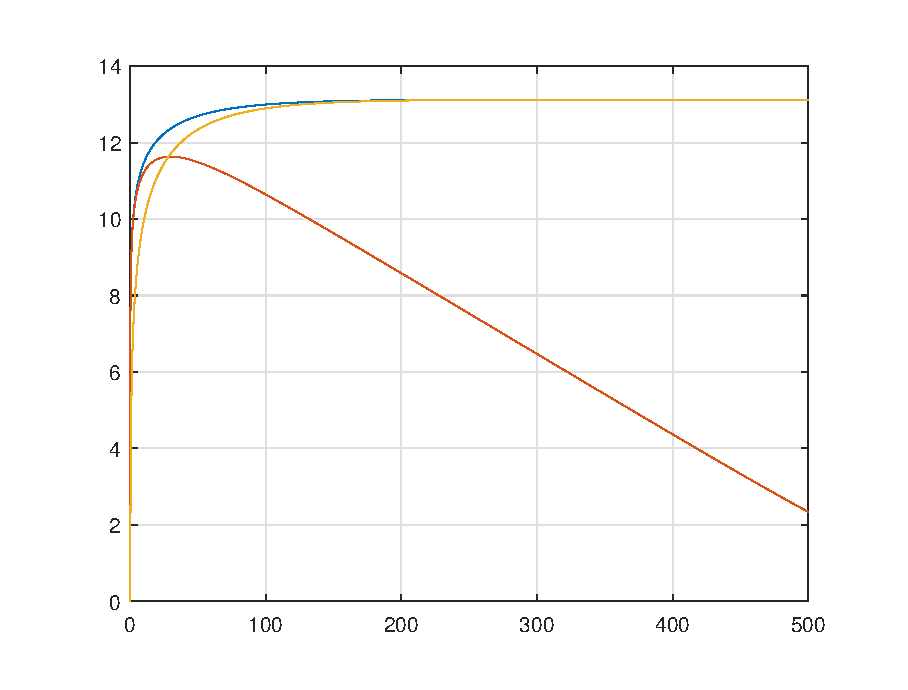
\includegraphics[width=1.5in,height=2in]{logalphazero.eps}}
	\qquad
	{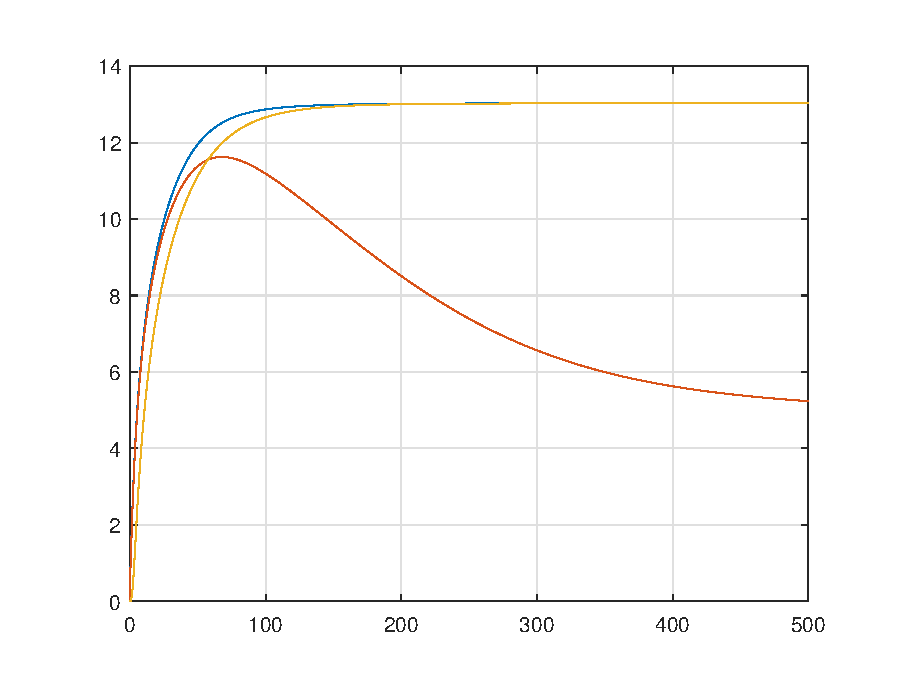
\includegraphics[width=1.5in,height=2in]{log075.eps}}
	\qquad
	{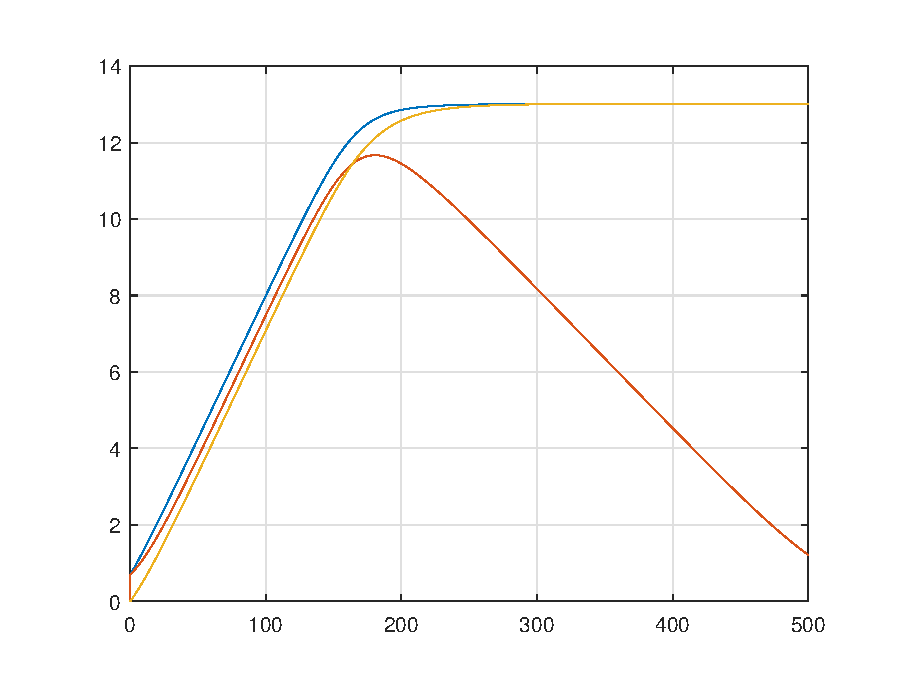
\includegraphics[width=1.5in,height=2in]{log1.eps}}
	%{\includegraphics[width=2in,height=2in]{Fig3.eps}}
	\end{center}
	%\begin{center}
	\caption{Logarithm of affected, infected and removed cases under $\gamma=0.05$  and $K=500.000$. Left, $\alpha=0$ and $\beta=10000$. Middle, $\alpha=0.75$ and $\beta=2$. Right, $\alpha=1$  and $\beta=0.125$}
	%\end{center}
	\label{log075}
\end{figure}

\bigskip

\begin{figure}
\begin{center}
%\subfloat [Second-chance model and absolute standard normal]
{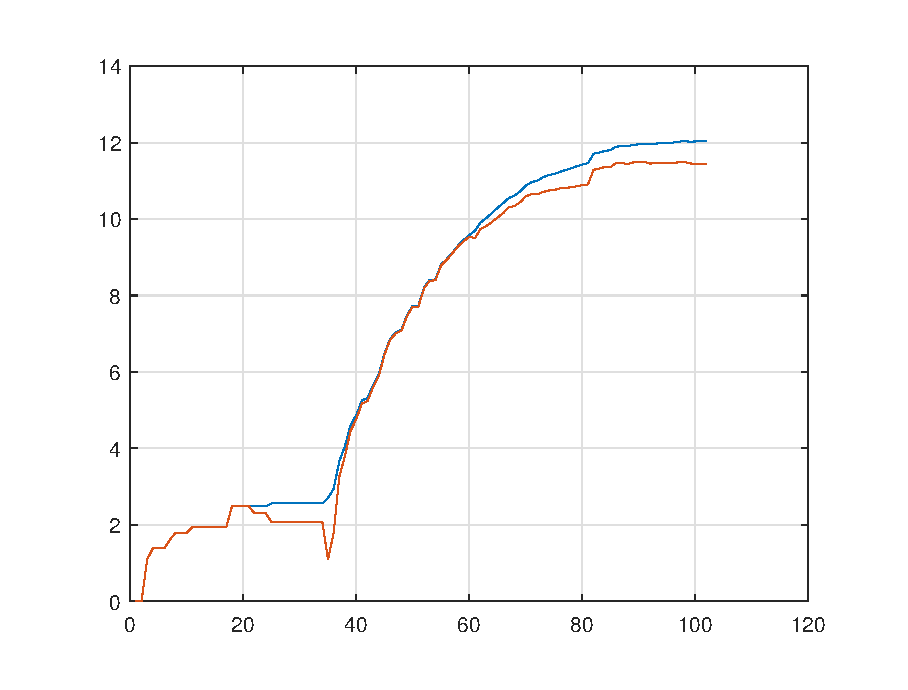
\includegraphics[width=1.5in,height=2in]{francelog.eps}}
 \qquad
{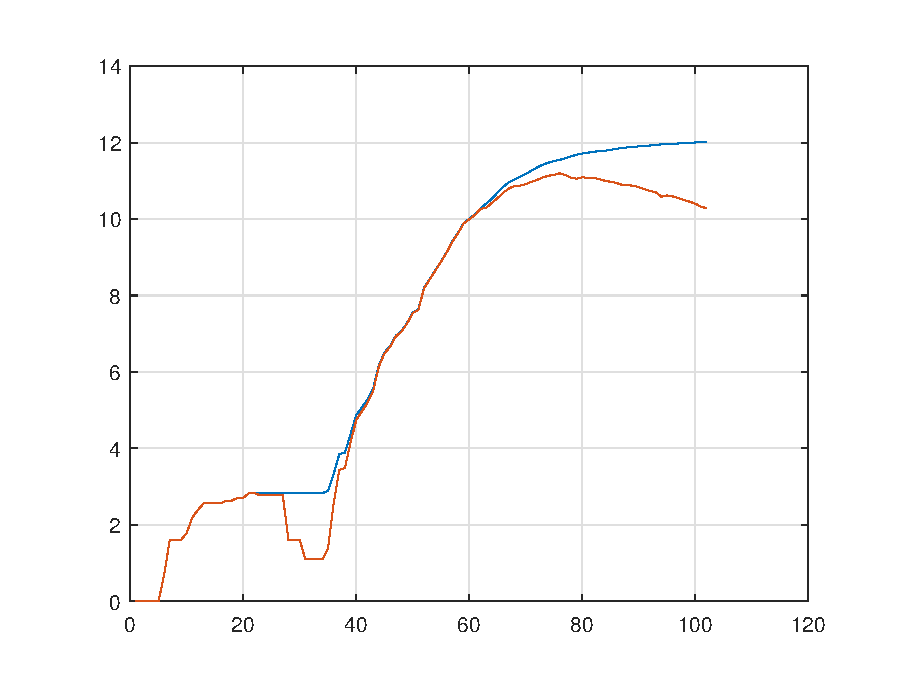
\includegraphics[width=1.5in,height=2in]{germany.eps}}
 \qquad
{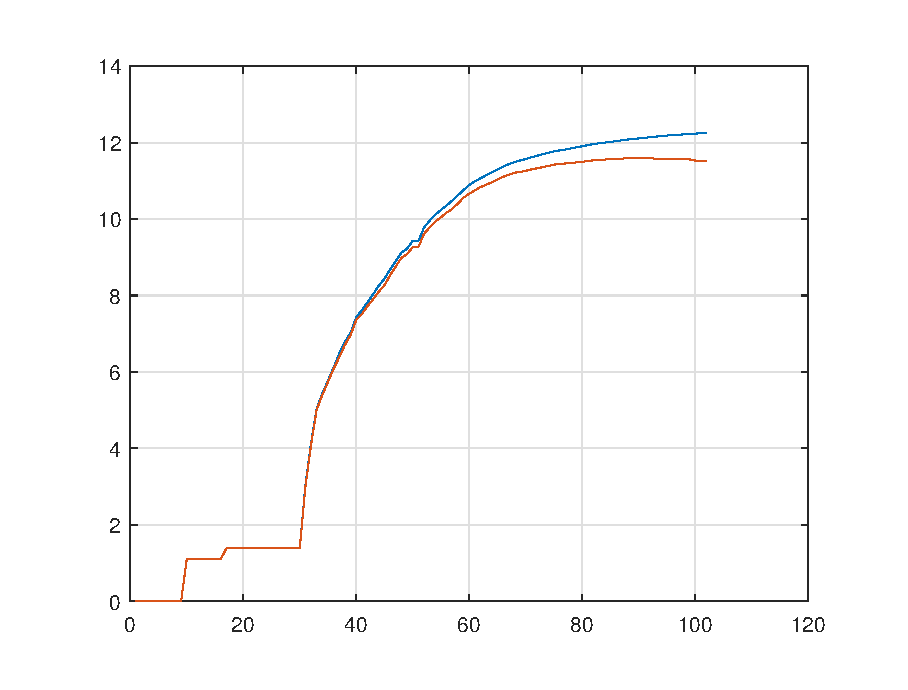
\includegraphics[width=1.5in,height=2in]{italy.eps}}
%{\includegraphics[width=2in,height=2in]{Fig3.eps}}
\end{center}
%\begin{center}
\caption{Logarithm of affected and infected cases, March to June 2020. Left, France. Middle, Germany. Right, Italy}
%\end{center}
\label{france}
\end{figure}


\noindent {\bf Remark on the $R_0$ transition below $1$}. It is quite popular these days to welcome this transition, wrongly referred to as leaving behind exponential growth in favor of a period of recovery. This transition occurs at the moment when the number of infected cases is at a maximum, where care should be perhaps strengthened rather than relaxed. All graphs in the sequel show that the recovery period until the number of infected cases is at a safer low level "in the current wave", is long and slow.  The USA is at the transition point in early June, but if conditions stay stationary, the current wave is predicted to be still at unsafe levels in November. Germany and Italy are predicted to experience unsafe levels at least until the end of August.

\section{The role of $\alpha$ for finite populations}
Consider the solution to the SIR equations for $K=500.000$ and $\gamma=0.01$. For each value of $\alpha$ from $0$ to $1$ (inclusive), at intervals of $0.05$, $\beta$ is determined so that the maximal value of $Y$ is ${K \over 2}$. These $21$ solutions to the SIR equations are plotted in the left side of Figure (\ref{fromtimes}). It is apparent that $\alpha$ has a strong effect on the time it takes for the disease to become noticeable. The right side of Figure (\ref{fromtimes}) displays exactly the same data, shifted in time so as to start from the day when the number of affected cases $X$ reaches ${K \over 10}$. All $21$ functions are similar to each other, and no wonder there is a relatively high variability in the estimation of $\alpha$. This nuisance parameter is like a chemical catalyzer - important for the statistical analysis but not very relevant for the result.
\begin{figure}
	
	\begin{center}
		%\subfloat [Second-chance model and absolute standard normal]
		{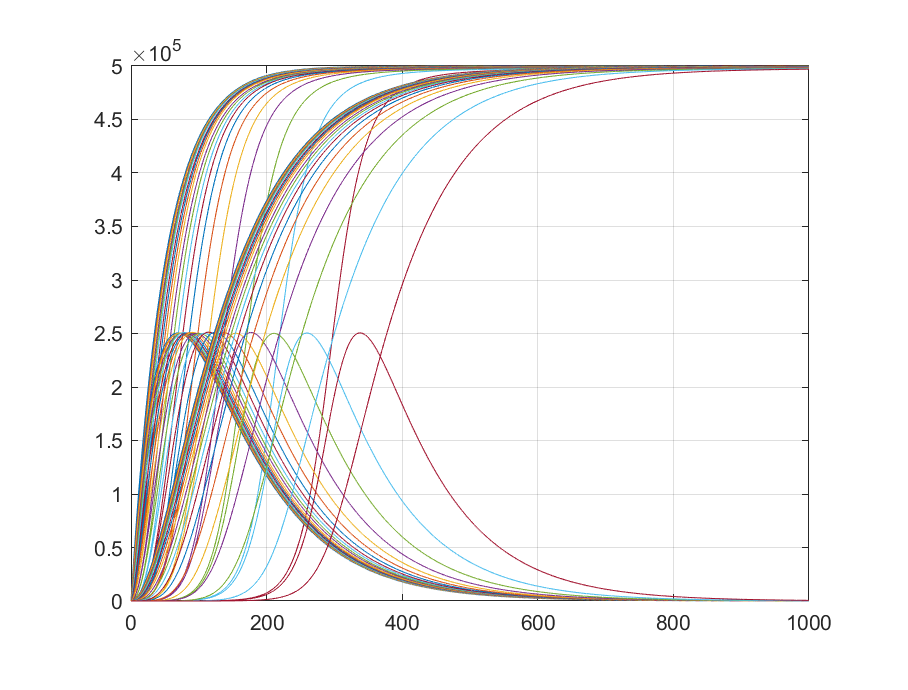
\includegraphics[width=2in,height=2in]{fromzero.eps}}
		\qquad
		{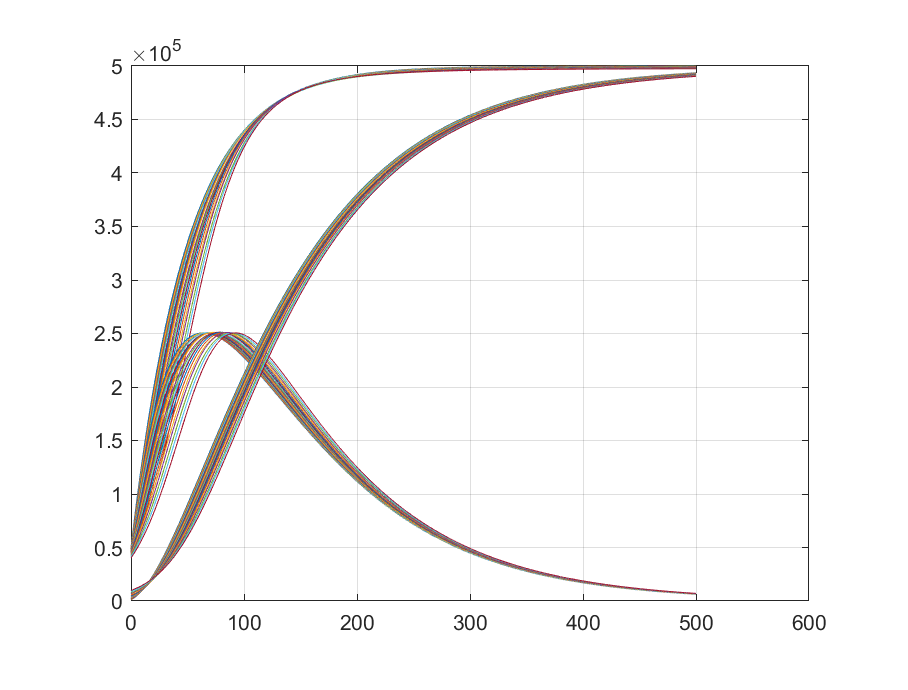
\includegraphics[width=2in,height=2in]{from5.eps}}
		\end{center}
		\begin{center}
	\caption{SIR functions with $K=500.000$ and $\gamma=0.01$. $\alpha$ ranges over $[0,1]$ and $\beta$ achieves that the maximal number of infected cases is ${K \over 2}$. Left, the SIR solutions. Right, the same functions shifted so as to start when the number of affected cases is ${K \over 10}$
	}
	\label{fromtimes}
	\end{center}
\end{figure}
	
	
	Initial data, that could have been informative in estimating $\alpha$, is generally unreliable. Hence, analysis is restricted to the data past a threshold on the number of affected cases $X$. The positive side is that the conclusions are then quite insensitive to this lack of knowledge about $\alpha$. The introduction of this rather diffuse $\alpha$ prevents spurious as-if accuracy in the estimation of the other parameters.
	
	In the benefit of focus, we refrain from studying further the possibilities opened by this section. Suffice to stay at this stage that $\log(\beta)$ comes out an almost perfectly linear function of $\alpha$. A subject for further study.
	
\section{Preliminary data handling and analysis} \label{preliminarysection}

Equation (\ref{DEforR}) expresses the reasonable premise that new removed cases are proportional to the number of infected cases. I.e., the cumulative number $R$ of removed cases should be proportional to the cumulative sum of currently infected cases. A linear regression with slope $\gamma$ and zero intercept should manifest this relationship. After checking that this is roughly so, the empirically measured affected cases $X$ are kept intact but its division into removed cases $R$ and infected cases $I$ is modified minimally so that the regression relation will hold. The method by which this pre-processing has been done can be found in the Appendix, together with an 8-country illustration of the effect of pre-processing. Figures
 %\ref{fig:brazil_sir_model_07_06_2020}, \ref{fig:germany_sir_model_07_06_2020}, \ref{fig:italy_sir_model_07_06_2020},
\ref{fig:belgium_sir_model_07_06_2020}-\ref{fig:usa_sir_model_07_06_2020} display on the right the raw and pre-processed data for a number of countries. This pre-processing regression provides interim estimates of $\gamma$ very close to the MLE estimate derived from the methods to be described.

The data of Italy and USA show close agreement between raw and pre-processed versions, with the pre-processed version smoothing relatively sharp jumps in the raw data.

The data of Brazil show close agreement, but still at an early stage in the epidemic.

The data of Germany and Switzerland show some disagreement in the number of infected cases. Regression pre-processing can be a tool for reverse engineering. It is apparent from the data that both countries failed to recognize recovered cases until March 25, and from then on Switzerland updated the number of recovered cases every week or so.

A similar reporting problem prevents proper analysis of the Swedish data, that updates the number of recovered cases seven times in the four months of Corona monitoring. It would have been interesting to watch more closely at the epidemic development in a country that imposed no regulatory measures.

The data of Belgium is of special interest. It has been announced that Belgium recorded as affected cases also those under doubt. As a result, it appears as if it holds record high deaths per million, and number of infected cases that is still growing on June 7th, unlike all its neighbors. Pre-processing is in sharp disagreement with the raw data, placing Belgium in the same standard stage as its neighbors, well past the transition to $R_0$ below $1$, and suggesting lethality not above standard European levels.

The data of Chile and France in Figure \ref{fig:chile_france_india_iran_07_06_2020} show drastic corrections in the number of recovered cases, rendering analysis difficult. Although Chilean raw and modified data show agreement when the last 10 days are omitted (Figure \ref{fig:chile_and_israel_25_05_2020}), the later drastic corrections place accuracy in doubt.

The data of Iran (Figure \ref{fig:chile_france_india_iran_07_06_2020}) and Israel (Figure \ref{fig:israel_peru_russia_turkey_07_06_2020}) show clear evidence of exit from steady conditions. However, Israel pre-processed data show (Figure \ref{fig:chile_and_israel_25_05_2020}) some disagreement with pre-processed data similarly to Germany and Switzerland, already before relaxing restrictions.

\bigskip
Before solving equations, a post-preliminary pre-processing validation of the basic model. If (\ref{DEforX}) is correct then $\log(\frac{newcases}{1-\frac{X}{K}})$ should be linear in $\log(I)$, with slope $\alpha$. "New cases" in a given day is the daily average in the week around the day. $K$ was roughly set as $2 \max(X)$ in the USA and as $1.1 \max(X)$ in Italy and Germany. Figure \ref{fig:linear_prediction_of_log_new_cases} displays $\log(\frac{newcases}{1-\frac{X}{K}})$ and the linear predictor.

\begin{figure}[ht]
    \begin{center}
%\subfloat [Second-chance model and absolute standard normal]
{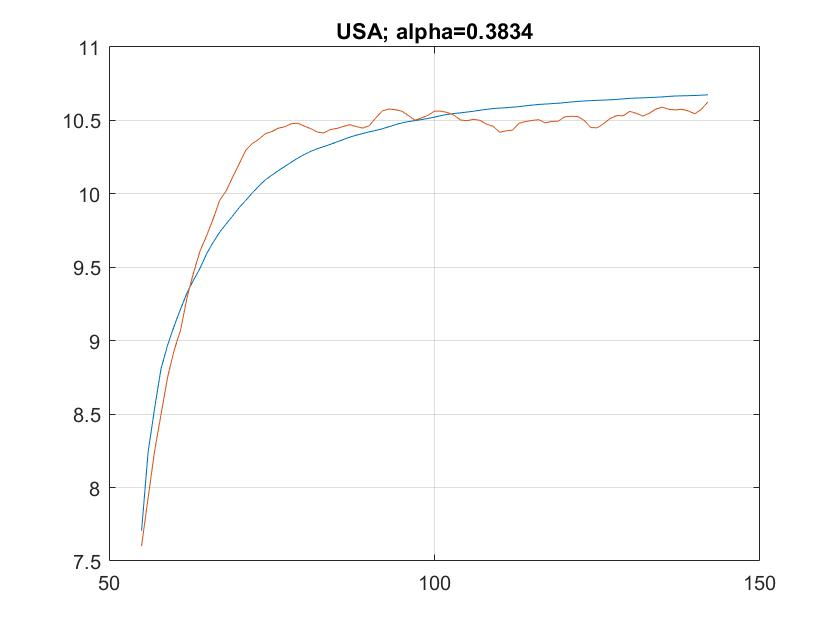
\includegraphics[scale = 0.13]{Paper_figs/regressionUSA.jpg}}
\qquad
{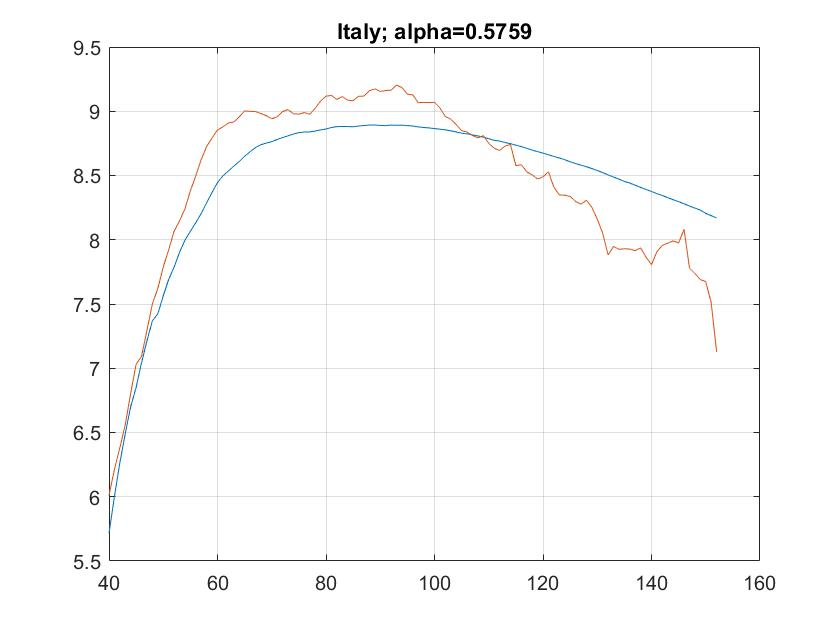
\includegraphics[scale = 0.13]{Paper_figs/regressionItaly.jpg}}
\qquad
{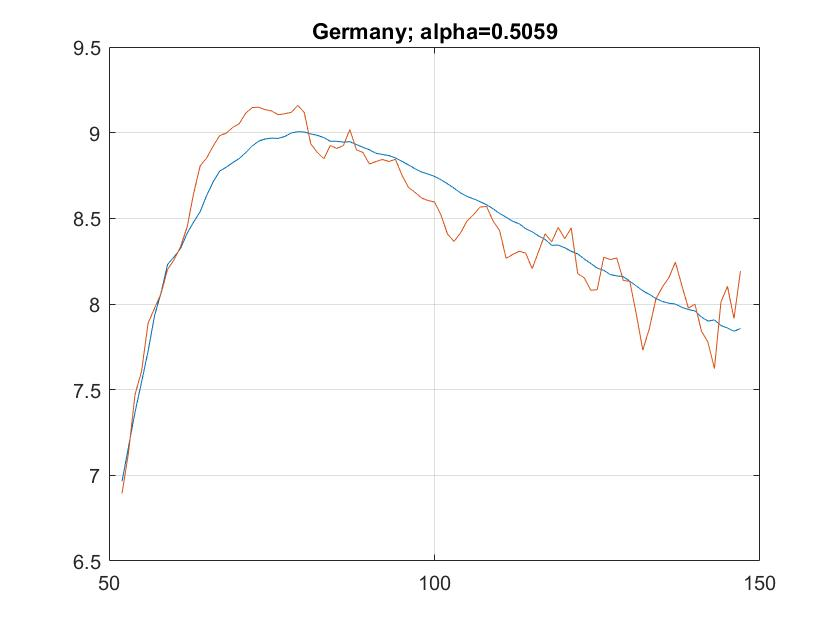
\includegraphics[scale = 0.13]{Paper_figs/regressionGermany.jpg}}
    \end{center}
    \caption{Linear regression of logarithmic affected-cases differential $\log(\frac{newcases}{1-\frac{X}{K}})$ on logarithmic infected cases. L: USA ($\alpha=0.3834$), C: Italy ($\alpha=0.5759$), R: Germany ($\alpha=0.5059$)}
    \label{fig:linear_prediction_of_log_new_cases}
\end{figure}    
%Equation (\ref{DEforI}) states that early in the epidemic $dI(t) \approx \beta (I(t))^\alpha$ or %${{(I(t))^{1-\alpha}} \over  {1-\alpha}} \approx \beta (t-t_0)$ for some $t_0$.
%The parameter $\alpha$ can thus be initially estimated by the one that maximizes the correlation %coefficient between $(I(t))^{1-\alpha}$ and time, on a properly chosen time interval. If this %correlation coefficient is close enough to $1$, the $\alpha$-model can be adopted, and the date $t_0$ %when the epidemic started, can be roughly assessed, together with $\alpha$ and $\beta$. Results are %omitted in favor of the analysis in the sequel, but
%the maximal achieved correlation coefficient exceeded $0.98$ in all nine countries tried.

\bigskip

Data for analysis consist of the empirical $X$ data and the $I$ and $R$ data modified by pre-processing. The next section will introduce parameter estimation of $K,\alpha, \beta,\gamma$ under the SIR equations.

\section{RTT and SDE applied to Covid19 2020} \label{RTTsection}

The paradigm to be adopted is that $\alpha$ is a (possibly location-dependent) characteristic of the condition, while $K$ is a local-scenario parameter that reflects behavior and regulatory measures. It is important to estimate all parameters jointly in order to obtain as accurate an estimate of $\alpha, \beta, \gamma$ as feasible. This will allow the calculation of $I_0$ in (\ref{Isub0}) as an estimated upper bound (corresponding to an infinite population) on the ongoing number of infected cases as well as of the slope of the linear functions in (\ref{slopes}), the condition incidence per unit time.

\bigskip

\noindent {\bf The RTT and SDE methods to solve differential equations with data subject to noise}. The relatively novel theoretical contribution of this report is the RTT method to mimic systems of deterministic differential equations by stochastic counterparts, conceptually different and simpler than the stochastic differential equations based on Diffusion processes. Both methods will be described and applied.

Parameter estimation ($\beta, \gamma, K, \alpha$) will be performed by the Random Time Transformation (RTT) method developed by Bassan, Marcus, Meilijson and Talpaz \cite{Bassanetal}, motivated by the notion of Skew Product in Ergodic Theory (see, e.g., Krengel \cite{Krengel}). These time transformations are a common method in Diffusion analysis and stochastic integration, as the semigroups of stopping times that embed Martingales and other processes into Brownian Motion (Doeblin \cite{Doeblin}, Skorokhod \cite{Skorokhod}, Monroe \cite{Monroe}, Dubins \& Schwarz \cite{DubSch}).

Unlike Diffusion methods that place noise vertically, the RTT method adopts the solution to the deterministic ODE, but considers it as evaluated at a random time process that advances on the average like chronological time. Thus, errors are horizontal. This random time is modelled in simplest practice as a Gaussian process (Brownian Motion or Ornstein-Uhlenbeck), but the first passage time distribution in Brownian Motion with drift will be implemented too. Whichever is chosen, it provides a likelihood model for the estimation of parameters inherent in the SIR (or otherwise) system of ODE. The differential terms $g(I(t)) (1 - X(t)/K)$ and $I(t)$ in equations (\ref{DEforX},\ref{DEforR}) identify the Jacobian term in the likelihood function, for the application of MLE, including both point estimates and standard errors.

For the application of SDE, the differential functions in (\ref{DEforX})-(\ref{DEforR}) identify the drift terms. Appendix 2 provides an argument that the closest SDE model to RTT has diffusion term proportional to the drift term. This model will be adopted. Furthermore, it will be assumed that a day is a short enough interval of time, so drift and diffusion can be considered constant, and the transition densities are simply Gaussian densities instead of the technically involved solutions via Fokker-Planck equations. For details on stochastic integrals and Fokker-Planck or Kolmogorov forward equations, consult Karatzas and Shreve \cite{Karatzas}.

\bigskip

Empirical data consist of $(X_1,R_1), (X_2,R_2), \dots, (X_n, R_n)$, from which the infected case totals $I_j=X_j-R_j$ can be inferred and then modified if needed, as described in Section (\ref{preliminarysection}.)
The sequences $X$ and $R$ are assumed or forced to be non-decreasing.

\bigskip

\noindent {\bf Time calibration determine $\beta$ and $\gamma$}. Whichever method is used (RTT with Gaussian increments, RTT with first-passage increments or SDE), these two parameters will be fitted "mechanically" (as opposed to "statistically") so that the feasible solutions of equations (\ref{DEforX})-(\ref{DEforR}) to be considered, that automatically start with $(X_1, R_1)$, will end exactly with $(X_n, R_n)$. \textit{I.e,}, the likelihood models will apply for the estimation of $K$ and $\alpha$ only, with $\beta$ and $\gamma$ expressed as functions of $K$ and $\alpha$.

\bigskip

The plan to be pursued is to solve the system above of ODE globally, as adequately as feasible, and if this plan succeeds and produces smooth, calculable, functions $(x,r,i)$ that tightly fit the empirical data, it will provide a prediction of the maximal future damage $K$ that $X$ will sustain, as well as of the timing of the transition from increasing to decreasing number of infected cases, or warn that such a transition is not due to happen in the foreseeable future. Furthermore, these functions, that may involve newly defined parameters that epidemiologists have no classical interpretation for, may replace the sparse and noisy empirical data for standard analysis.

No attempt will be made to solve the SIR system analytically. Instead, a small increment of time $\delta={1 \over M}$ is set, and the ODE is solved numerically as a difference equation. Interpreting as time the indices of the empirical data, $M=100$ is a reasonable choice. Numerical methods other than the na\"{i}ve choice (\ref{thesolution}) to solve differential equations may be substituted, of which the most obvious is to apply $i$ and $1 - \frac{x}{K}$ in the RHS of (\ref{thesolution}) evaluated at $j-{1 \over 2}$ instead of $j-1$. It only makes a negligible difference. The overly exact choice $M=100$ reduced the need to address this issue.

\bigskip

Fix the parameters $\beta, \gamma, K$ and the function $g$, initiate functions $x$ and $r$ as $X_1$ and $R_1$ respectively, initiate $i$ as $X_1-R_1$ and proceed with the definition for $j \ge 2$
\begin{eqnarray}
x(j)&=&x(j-1)+\beta g(i(j-1))(1-{{x(j-1)} \over K}) \delta \nonumber \\
r(j)&=&r(j-1)+\gamma i(j-1) \delta \nonumber \\
i(j)&=&x(j)-r(j) \label{thesolution}
\end{eqnarray}


As introduced above, the RTT idea works with horizontal errors:

\bigskip
Define the {\em random time trajectory} as starting at $T_1(1)=1, T_2(1)=1$. For $2 \le m \le n-1$, let $T_1(m)$ be defined by $x({{T_1(m)} \over \delta}) = X_m$ and $T_2(m)$ by $r({{T_2(m)} \over \delta}) = R_m$. As for $m=n$, solve for $\beta$ and $\gamma$ so that $T_1(n)=T_2(n)=n$.

Define $\Delta_1(m)=T_1(m+1)-T_1(m)$ and $\Delta_2(m)=T_2(m+1)-T_2(m)$, for $1 \le m \le n-1$, as the (mean-$1$) increments of the $T_1$ and $T_2$ processes.

\bigskip

If population size $N$ was substituted for $K$ and the identity function for $g$, work is over. For quality-of-fit sanity check, plot the $(x,r,i)$ solution with the $(X,R,I)$ data, that agree at both time endpoints.

Else, $K$ and $\alpha$ are considered as free parameters, to be estimated from the data.

\bigskip

\noindent {\bf The likelihood function induced by the RTT method and SDE methods}. For simplicity, view the incremental times $(\Delta_1(m),\Delta_2(m))$
as observations from a bivariate mean-zero Gaussian distribution, and let $\Sigma$ be their empirical covariance matrix. Up to a multiplicative constant, the normal density evaluated at these data is $(\det(\Sigma))^{-{{n-1} \over 2}}$.

Alternatively, view the processes $T_1(m)-m$ and $T_2(m)-m$ as bivariate Gaussian random walk bridges.
These two models yield equivalent Gaussian density functions. As a result, the simpler as-if i.i.d. formulation is adopted. For details on the random walk bridge covariance function and its inverse, consult \cite{Cuadras}. 

The diffusion and random time methods are similar. Appendix 2 expands on this similarity and introduces the diffusion method to solve the current problems.


\bigskip

The random time likelihood function for the RTT model is obtained by multiplying the random time density described above by the Jacobian of the transformation. This can be easily seen to be the ratio of $1$ over the product over the sample of the differential terms $\beta g(X_m-R_m)(1-X_m/K)$ and $\gamma (X_m-R_m)$, perhaps evaluated at
${{X_m+X_{m-1}} \over 2}$ and ${{R_m+R_{m-1}} \over 2}$ instead of $X_m$ and $R_m$. It doesn't make a difference, as the main regularization role of the Jacobian is to penalize the Gaussian Least Squares into producing smoother solutions.

\bigskip

The parameters $K$ and $\alpha$ are MLE-estimated by maximizing the logarithm of this profile likelihood function, and their standard errors (and correlation coefficient, if needed) are estimated as usual, via the empirical Fisher information.


\section{Covid19 analysis in six countries} \label{Covid19}

\begin{table}
\begin{center}
\begin{tabular}{l|ccccccc|r}
Country & $\alpha$ & $\beta$ & $\gamma$ & $\sigma_X $ & $ \sigma_R$ & $\rho$ & $K$ & $X_{max}$ \\ \hline
Belgium & $0.497$ & $16.06$ & $0.014$ & $0.296$ & $0.071$ & $0.240$ & $61510$ & $59072$ \\
Brazil  & $0.849$ & $0.57$ & $0.046$ & $0.255$ & $0.148$ & $0.578$ & N/A & $672846$ \\
%Chile   & 0.48 & 1.2318 &0.0450 &  55 &  113 & 50 & 0.9897 &  \\
%France  & 0.91 & 0.0025 &  0.0278& 38 & 72 & 1 & 0.9973 &  \\
Germany & $0.382$ & $131.00$ & $0.070$ & $0.343$ & $0.044$ & $0.127$ & $198917$ & $185450$ \\
%Israel & 0.01 &  292.61 & 0.0379 & 57 &  84& 59 & 0.9870 & \\
Italy  & $0.605$ & $9.97$ & $0.030$ & $0.193$ & $0.079$ & $0.410$ & $246234$ & $234801$ \\
Switzerland & 0.586 & 10.8 & 0.067 & 0.228  & 0.535 & 0.252 & 31575&      30956	    \\
USA    & $0.246$  & $1380.26$ & $0.011$ & $0.118$ & $0.023$ & $0.192$ & $3370399$ & $1920061$ \\ \hline
\end{tabular}
\caption{
Parameter estimation based on data until June 7, 2020
\label{tablejune7}
}
\end{center}
\end{table}

\bigskip

\begin{table}
\begin{center}
\begin{tabular}{l|ccccccc|r}
Country & $\alpha$ & $\beta$ & $\gamma$ & $\sigma_X $ & $ \sigma_R$ & $\rho$ & $K$ & $X_{max}$ \\ \hline
Italy  & $0.605$ & $9.99$ & $0.028$ & $0.168$ & $0.063$ & $0.377$ & $245431$ & $230158$ \\
USA    & $0.272$  & $478.24$ & $0.011$ & $0.143$ & $0.042$ & $0.294$ & $2699321$ & $1662302$\\ \hline
\end{tabular}
\caption{
Parameter estimation based on data until May 25, 2020
\label{tablemay25}
}
\end{center}
\end{table}


Section (\ref{preliminarysection}) hinged on the relation between raw and pre-processed data, as displayed by the right side of Figures  %\ref{fig:brazil_sir_model_07_06_2020}, \ref{fig:germany_sir_model_07_06_2020}, \ref{fig:italy_sir_model_07_06_2020},
(\ref{fig:belgium_sir_model_07_06_2020}-\ref{fig:usa_sir_model_07_06_2020}). The left side extends the solutions to SIR a few months into the future, and reports $95\%$ pointwise confidence intervals.

The analysis of the Brazilian data leads to a high value of $\alpha$, indicating fast, nearly exponential growth. Covid19 started relatively late, and analysis is brought as illustration only.

The analysis of the USA data indicates that the transition to $R_0$ below $1$ is around the end of monitoring for this report. Estimation on data until May 25th (Table \ref{tablemay25}) predicts maximal number of affected cases $K=2.7$ million, but it turns out to be an optimistic assessment, revised June 7th (Table \ref{tablejune7}) to $3.37$ million. According to these assessments, {\em if status quo of conditions is maintained}, the current wave of the epidemic would still be quite strong in December. Under the same conditions, Germany and Italy would see the epidemic nearly over by September.

The analysis of the Belgian data should be interpreted as a qualitative assessment that the epidemic progress in Belgium is essentially similar to that of its neighbors and casualties have been exaggerated, but it would not be reasonable to express quantitative conclusions.

\begin{figure}
\begin{center}
%\subfloat [Second-chance model and absolute standard normal]
{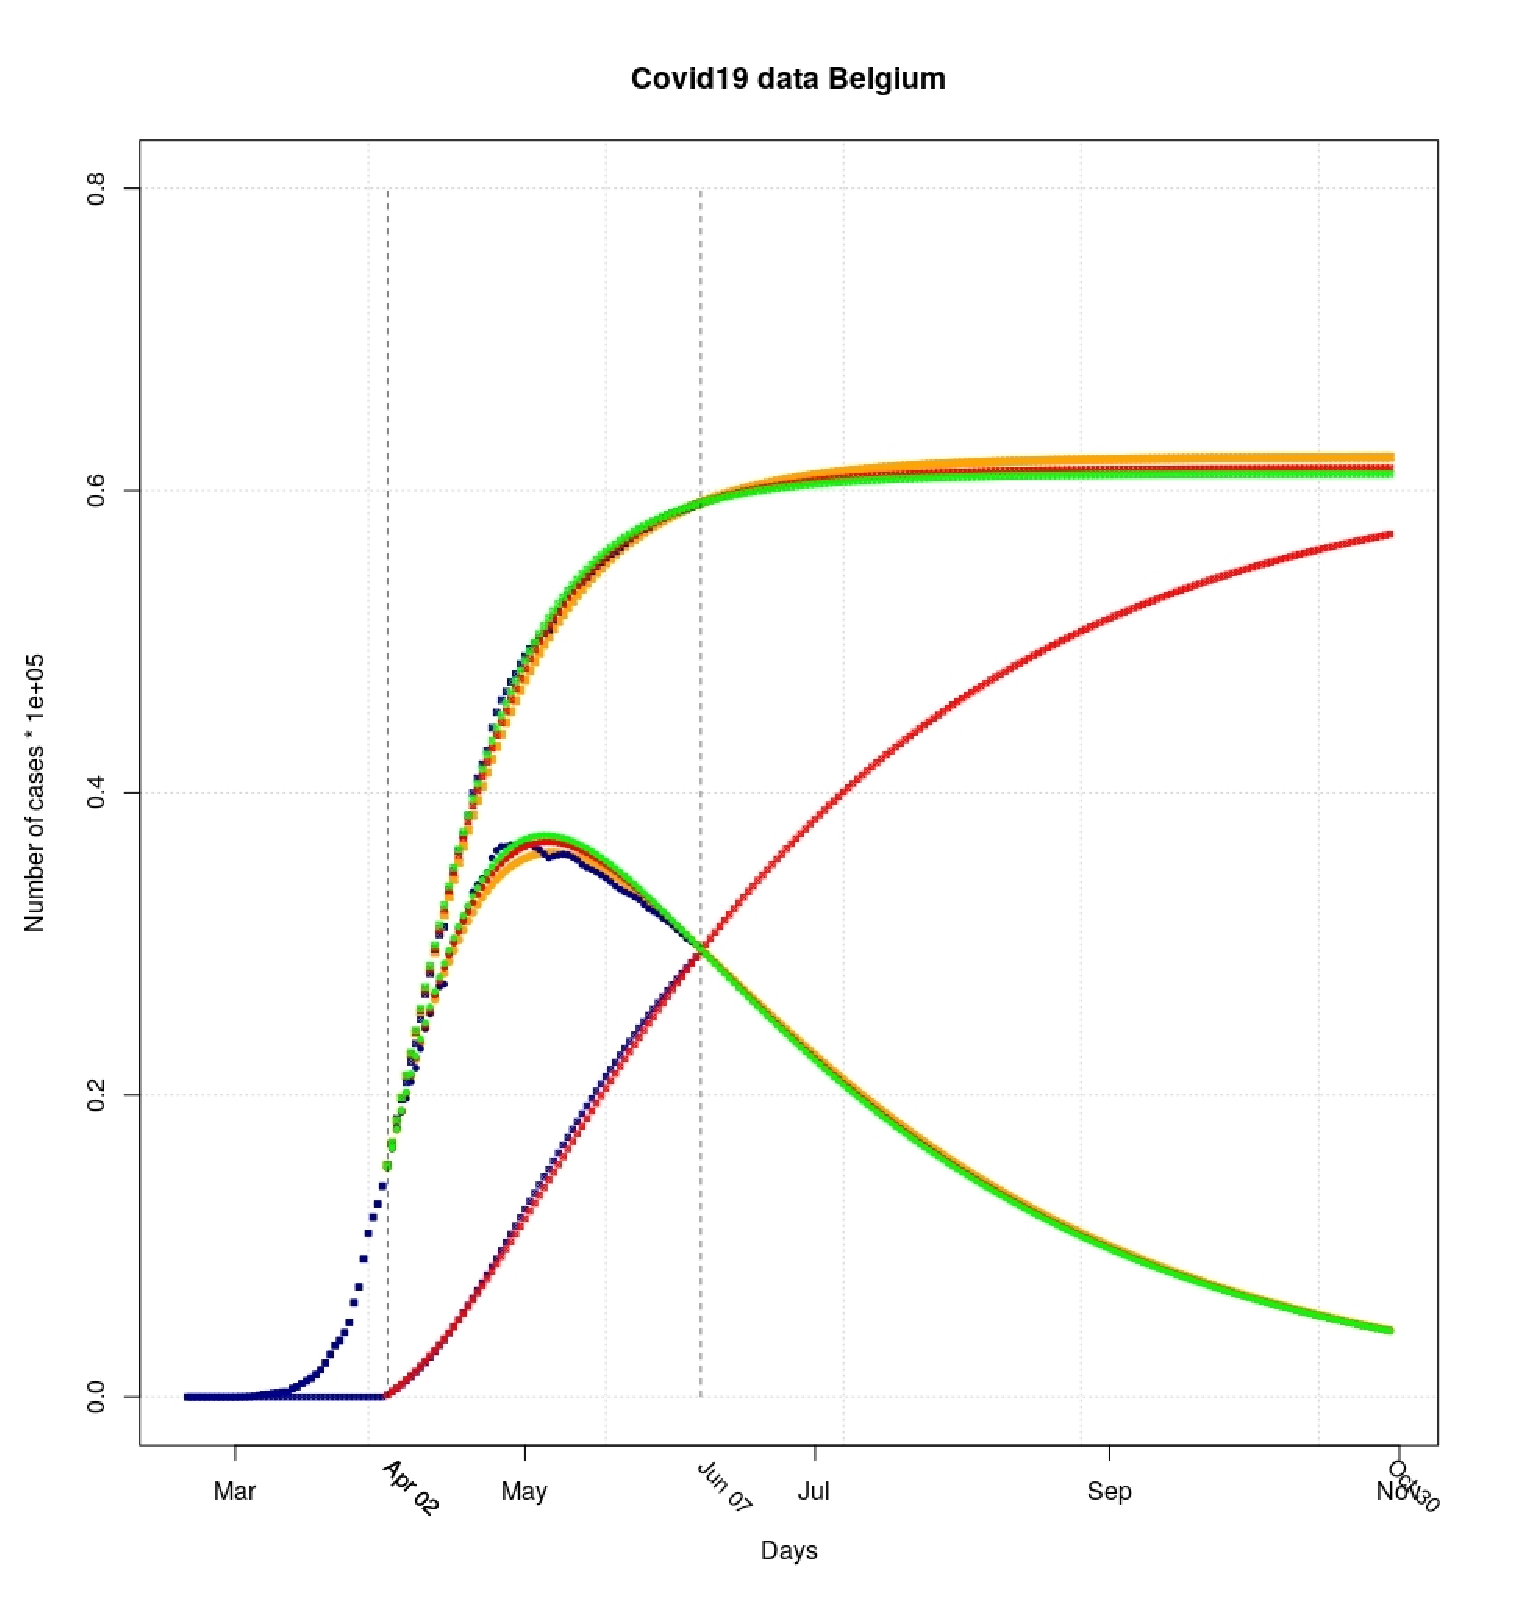
\includegraphics[width=2.5in,height=2in]{belgium_figure_a_07_06_2020.eps}}
\qquad
{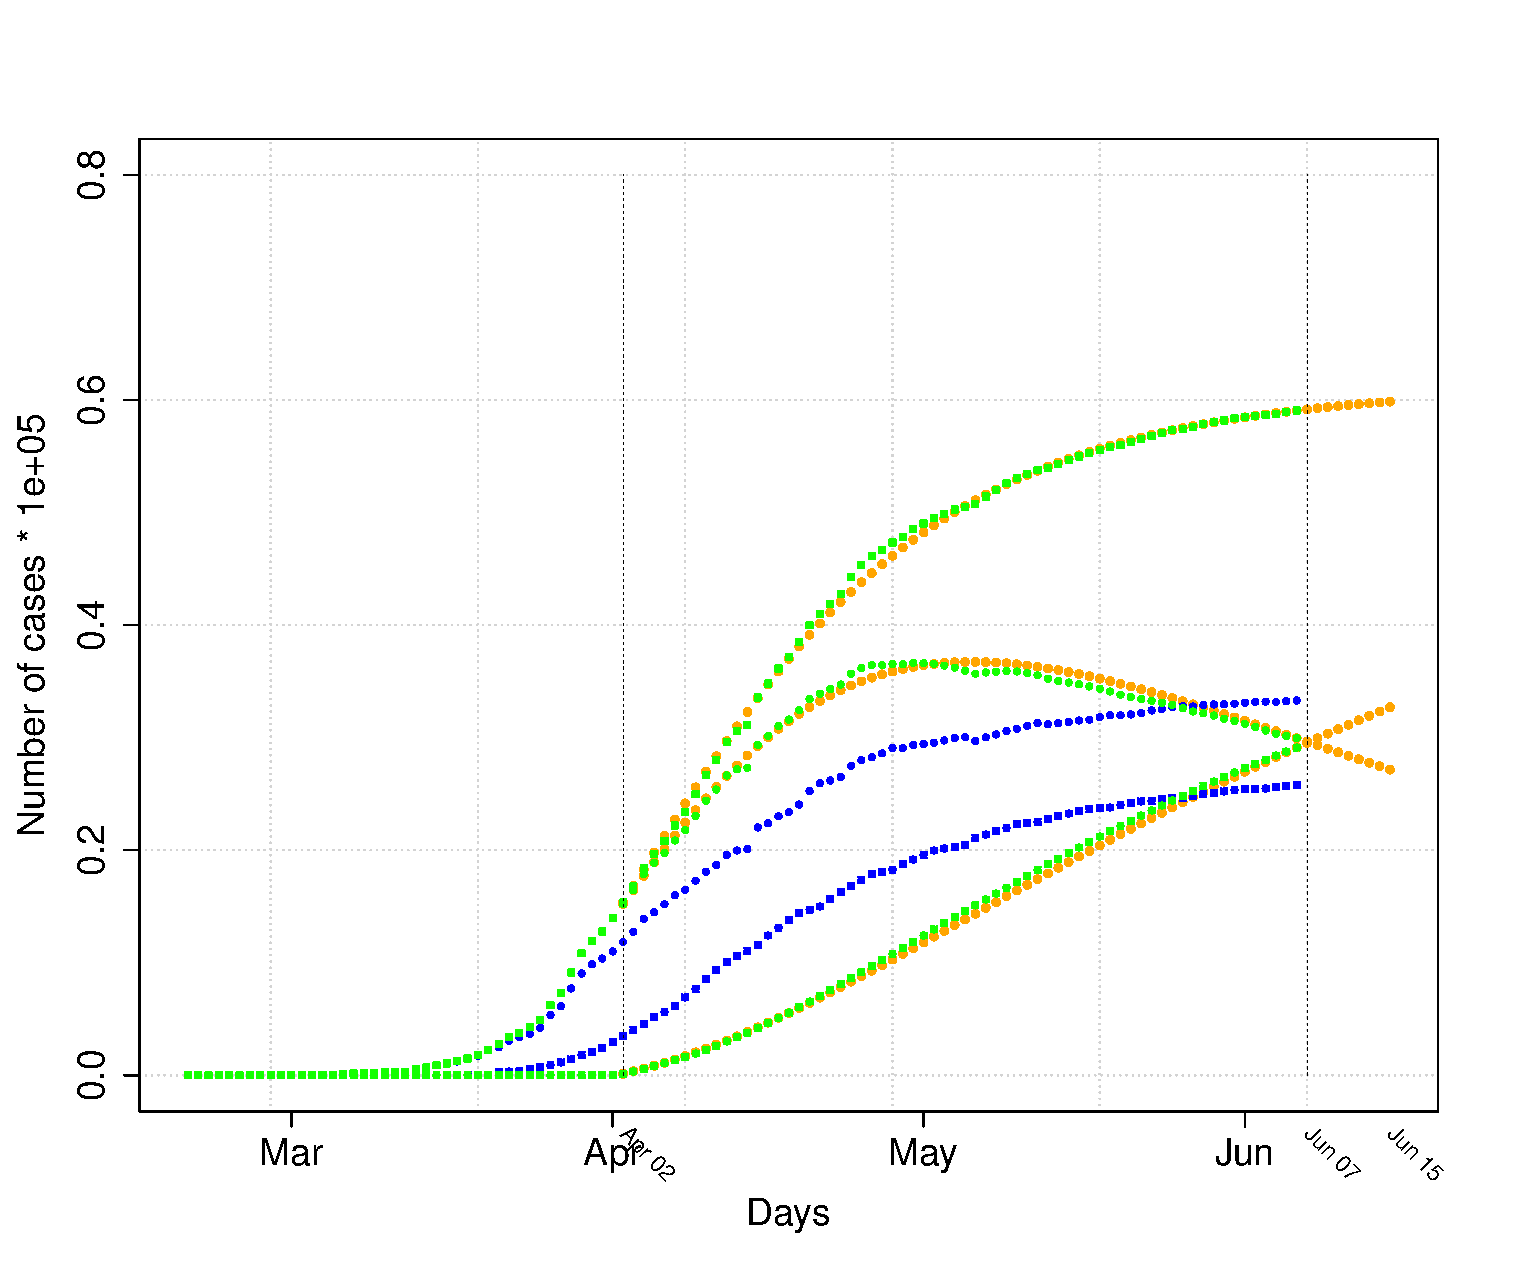
\includegraphics[width=2.5in,height=2in]{belgium_figure_b_07_06_2020.eps}}
\end{center}
\begin{center}
\caption{SIR model, data pre-processing and RTT solution, Belgium, March to June 2020
}
\label{fig:belgium_sir_model_07_06_2020}
\end{center}
\end{figure}

\begin{figure}
\begin{center}
%\subfloat [Second-chance model and absolute standard normal]
{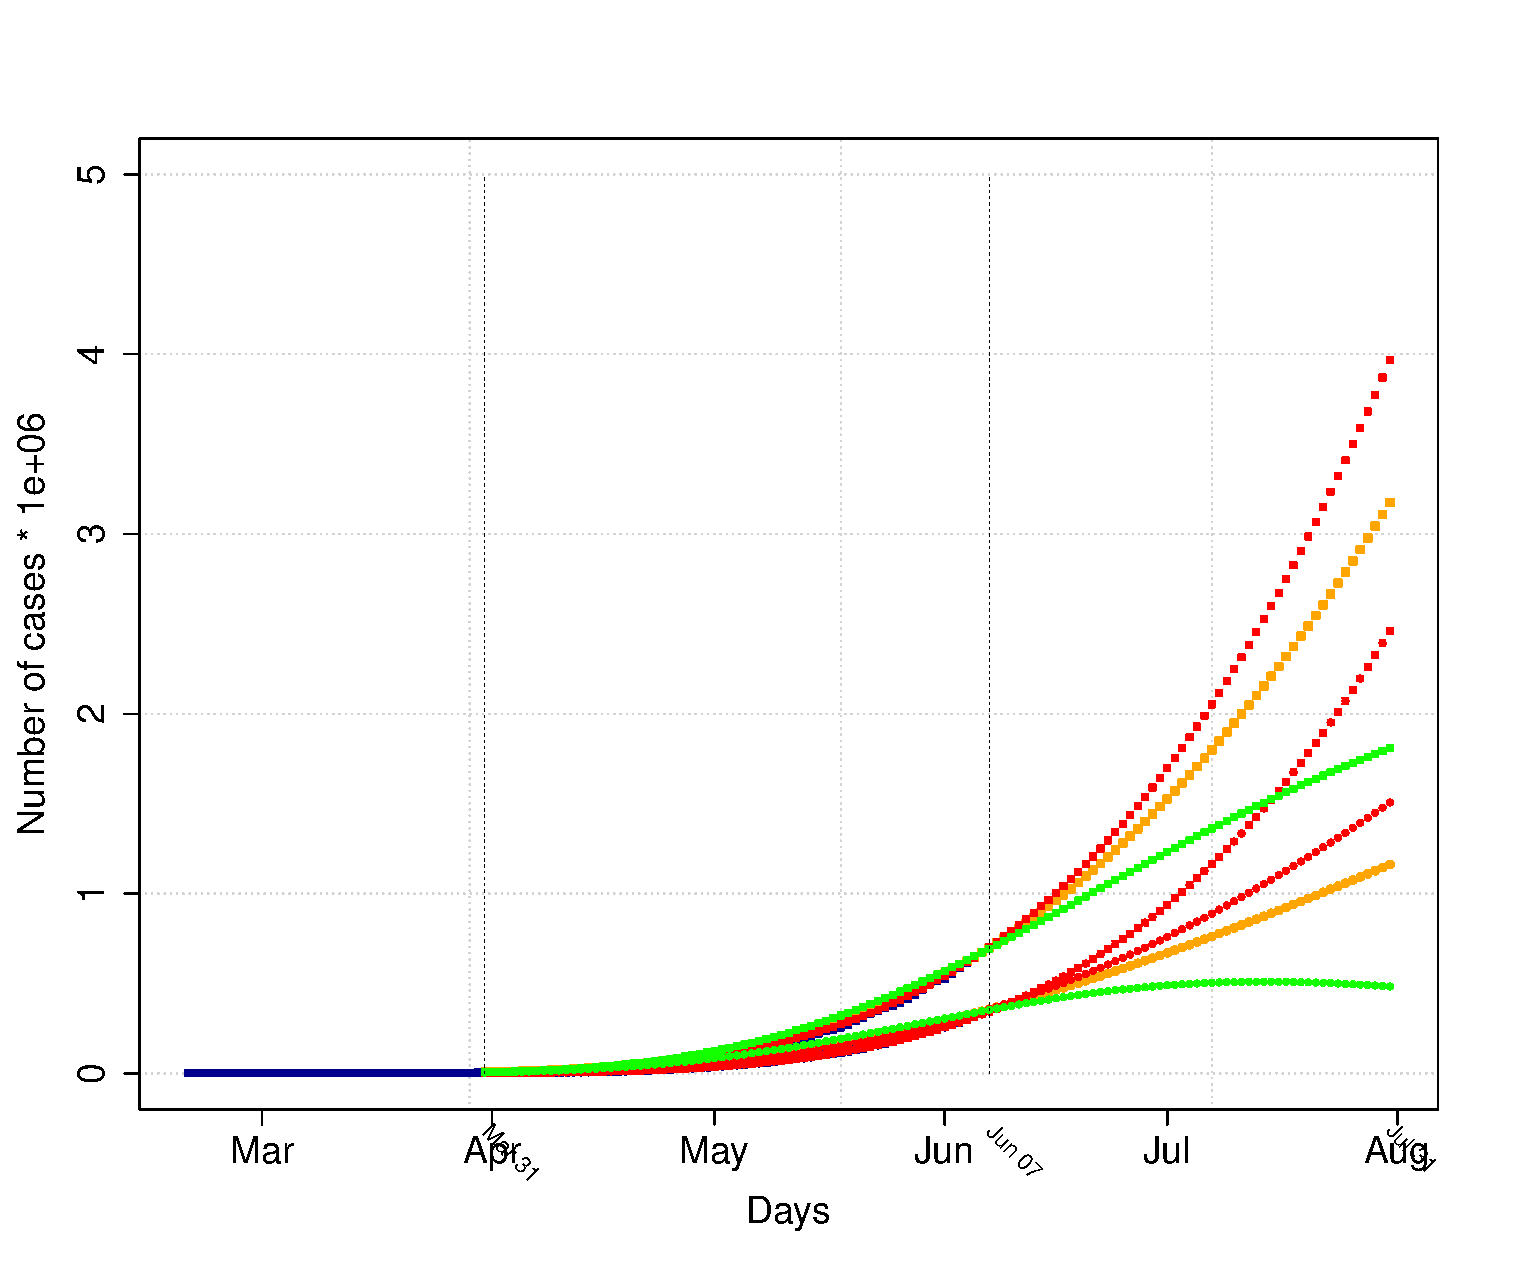
\includegraphics[width=2.5in,height=2in]{brazil_figure_a_07_06_2020.eps}}
\qquad
{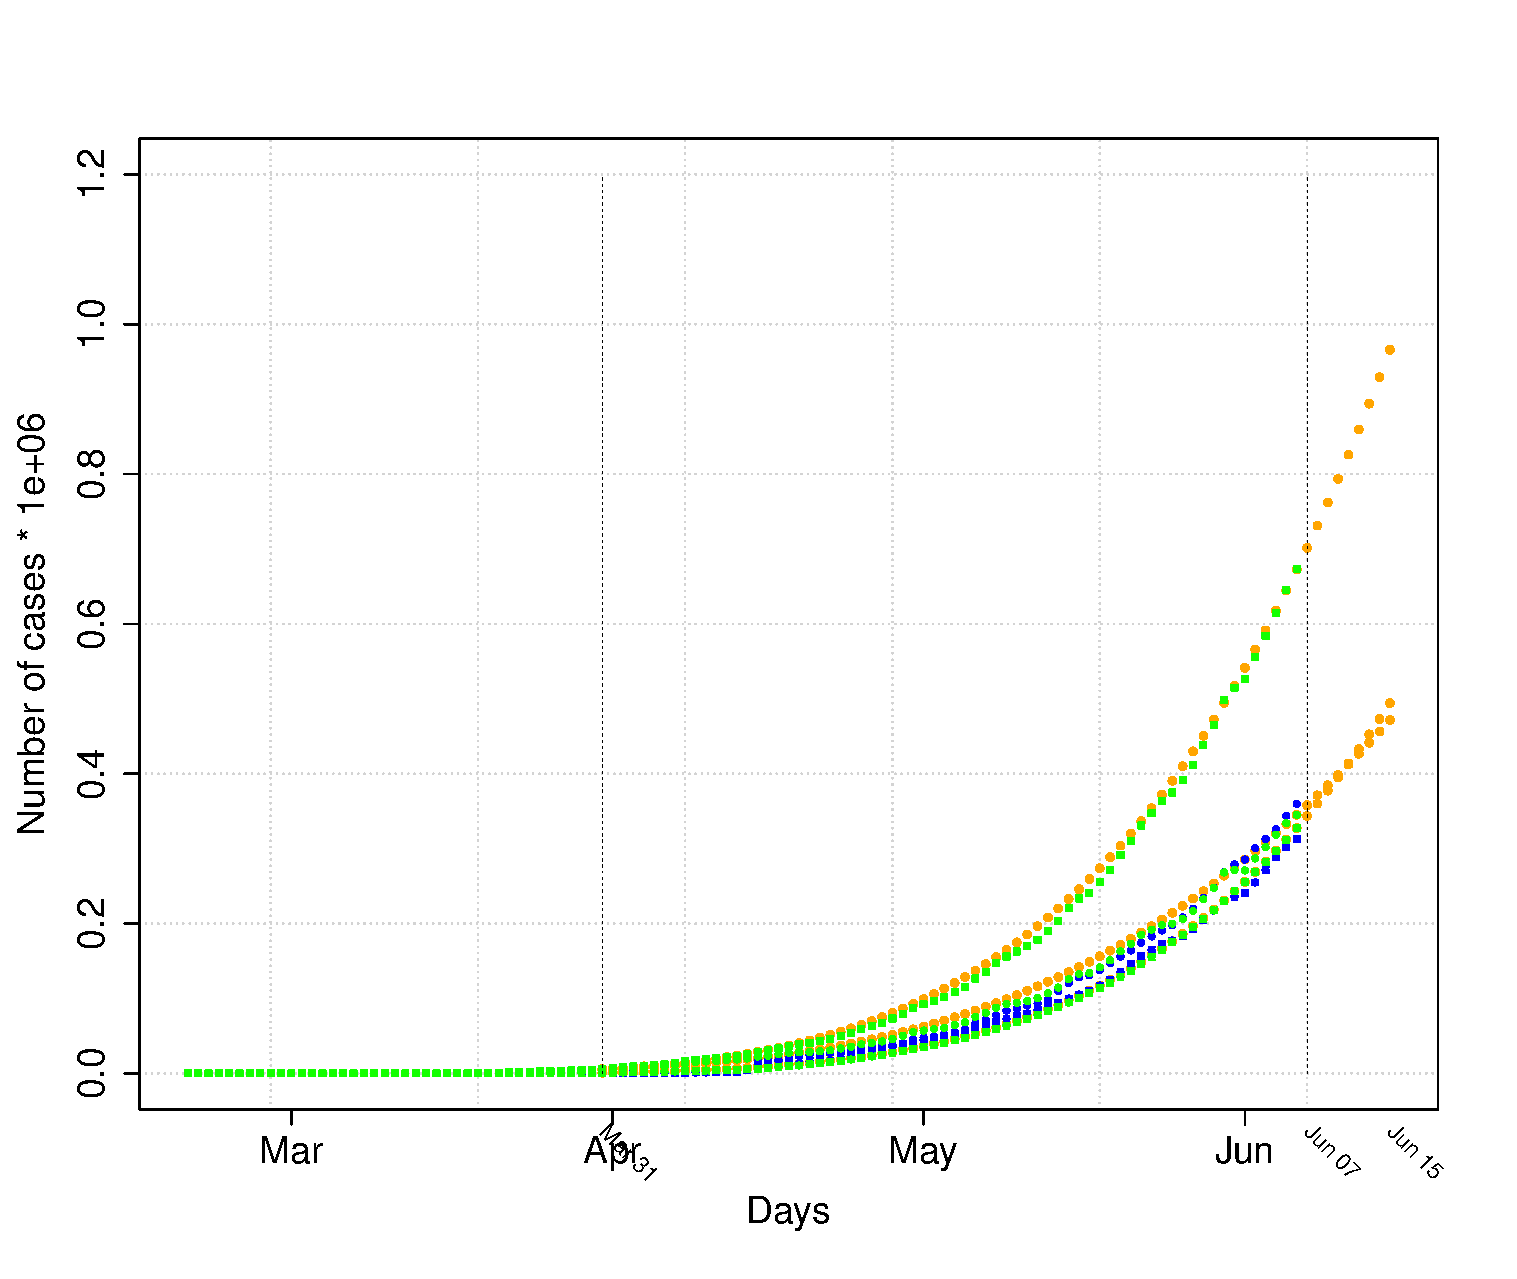
\includegraphics[width=2.5in,height=2in]{brazil_figure_b_07_06_2020.eps}}
\end{center}
\begin{center}
\caption{SIR model, data pre-processing and RTT solution, Brazil, March to June 2020
}
\label{fig:brazil_sir_model_07_06_2020}
\end{center}
\end{figure}

\begin{figure}
\begin{center}
%\subfloat [Second-chance model and absolute standard normal]
{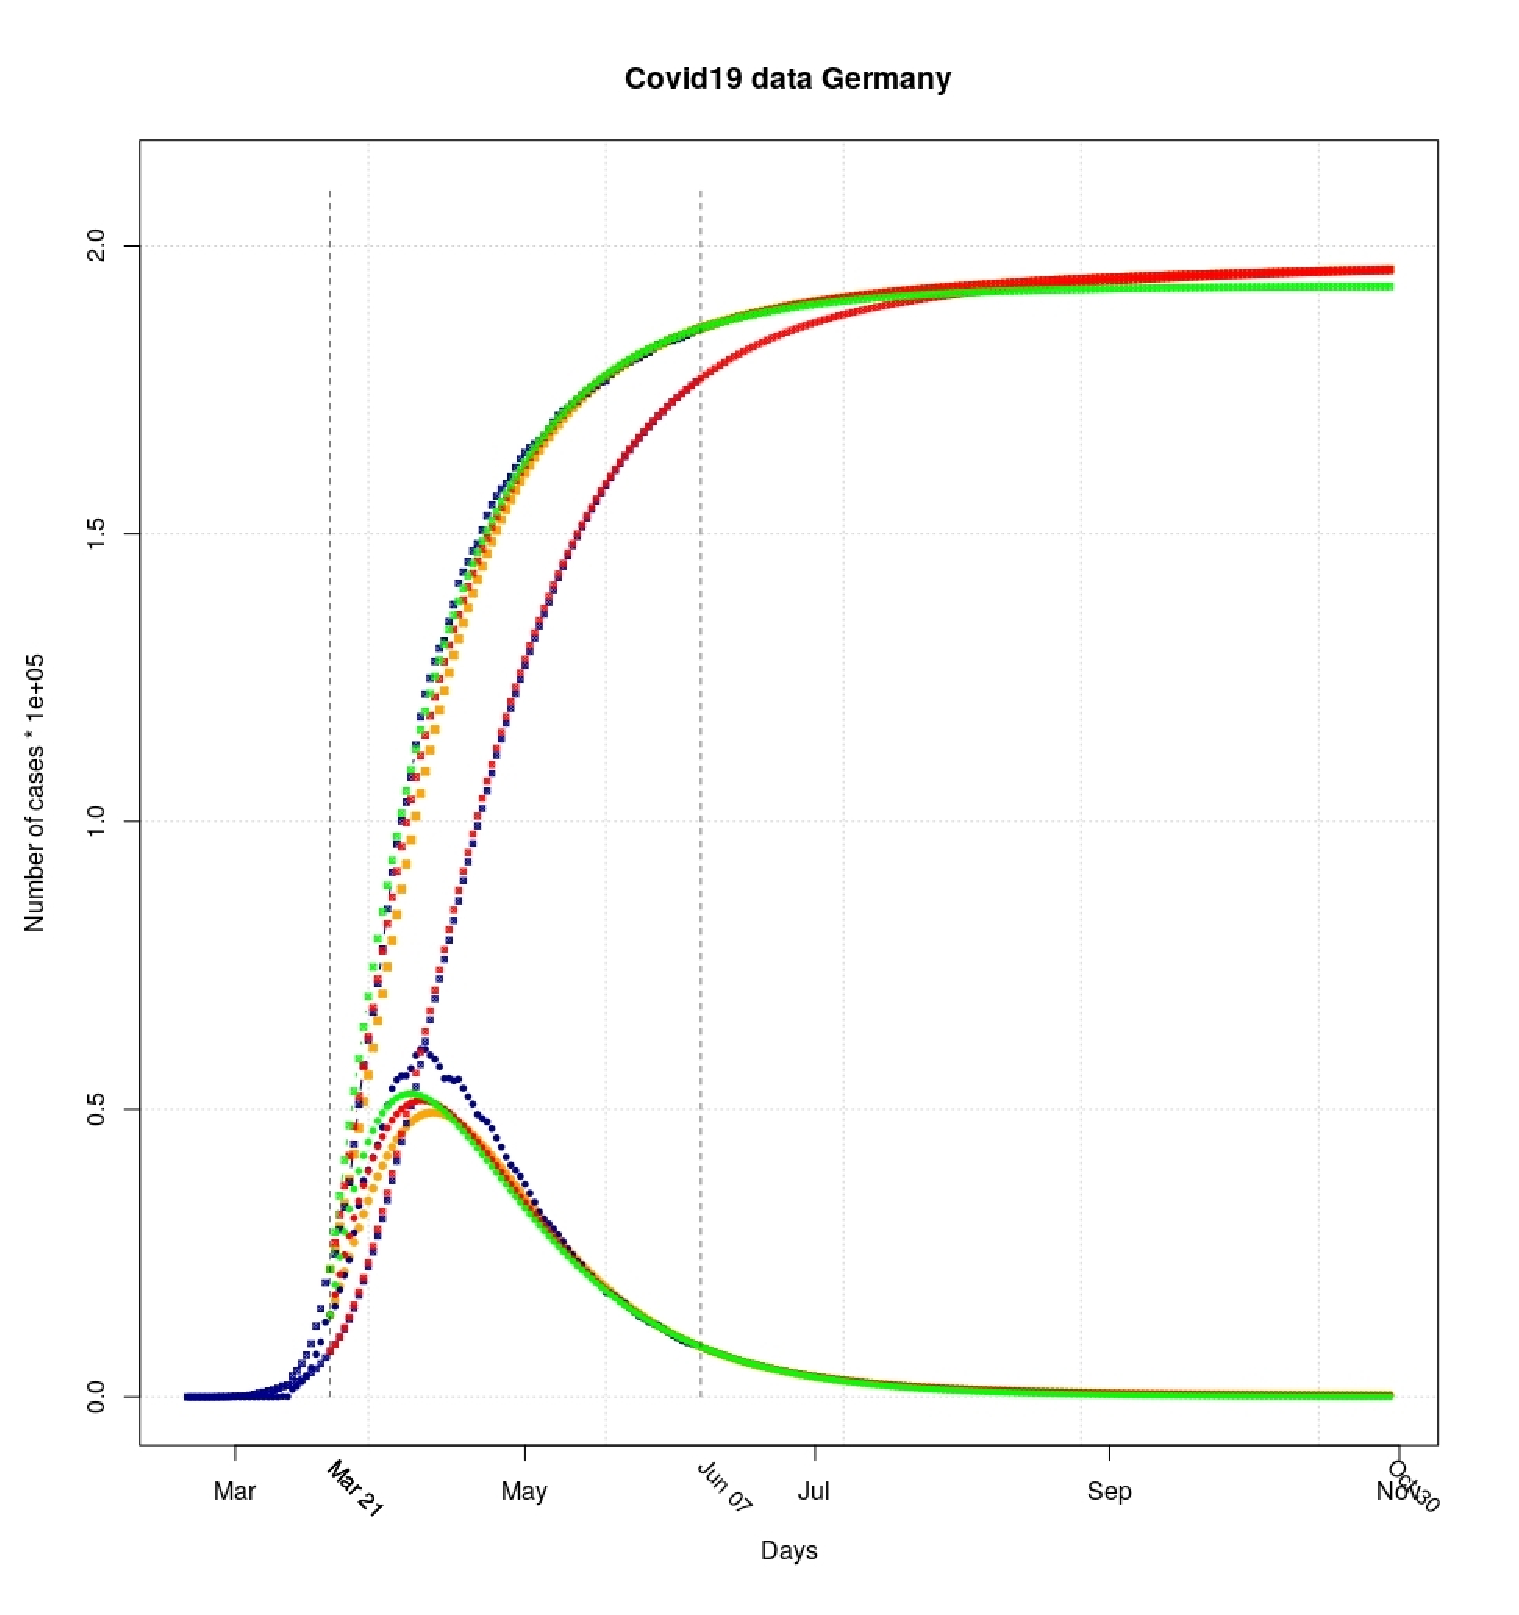
\includegraphics[width=2.5in,height=2in]{germany_figure_a_07_06_2020.eps}}
\qquad
{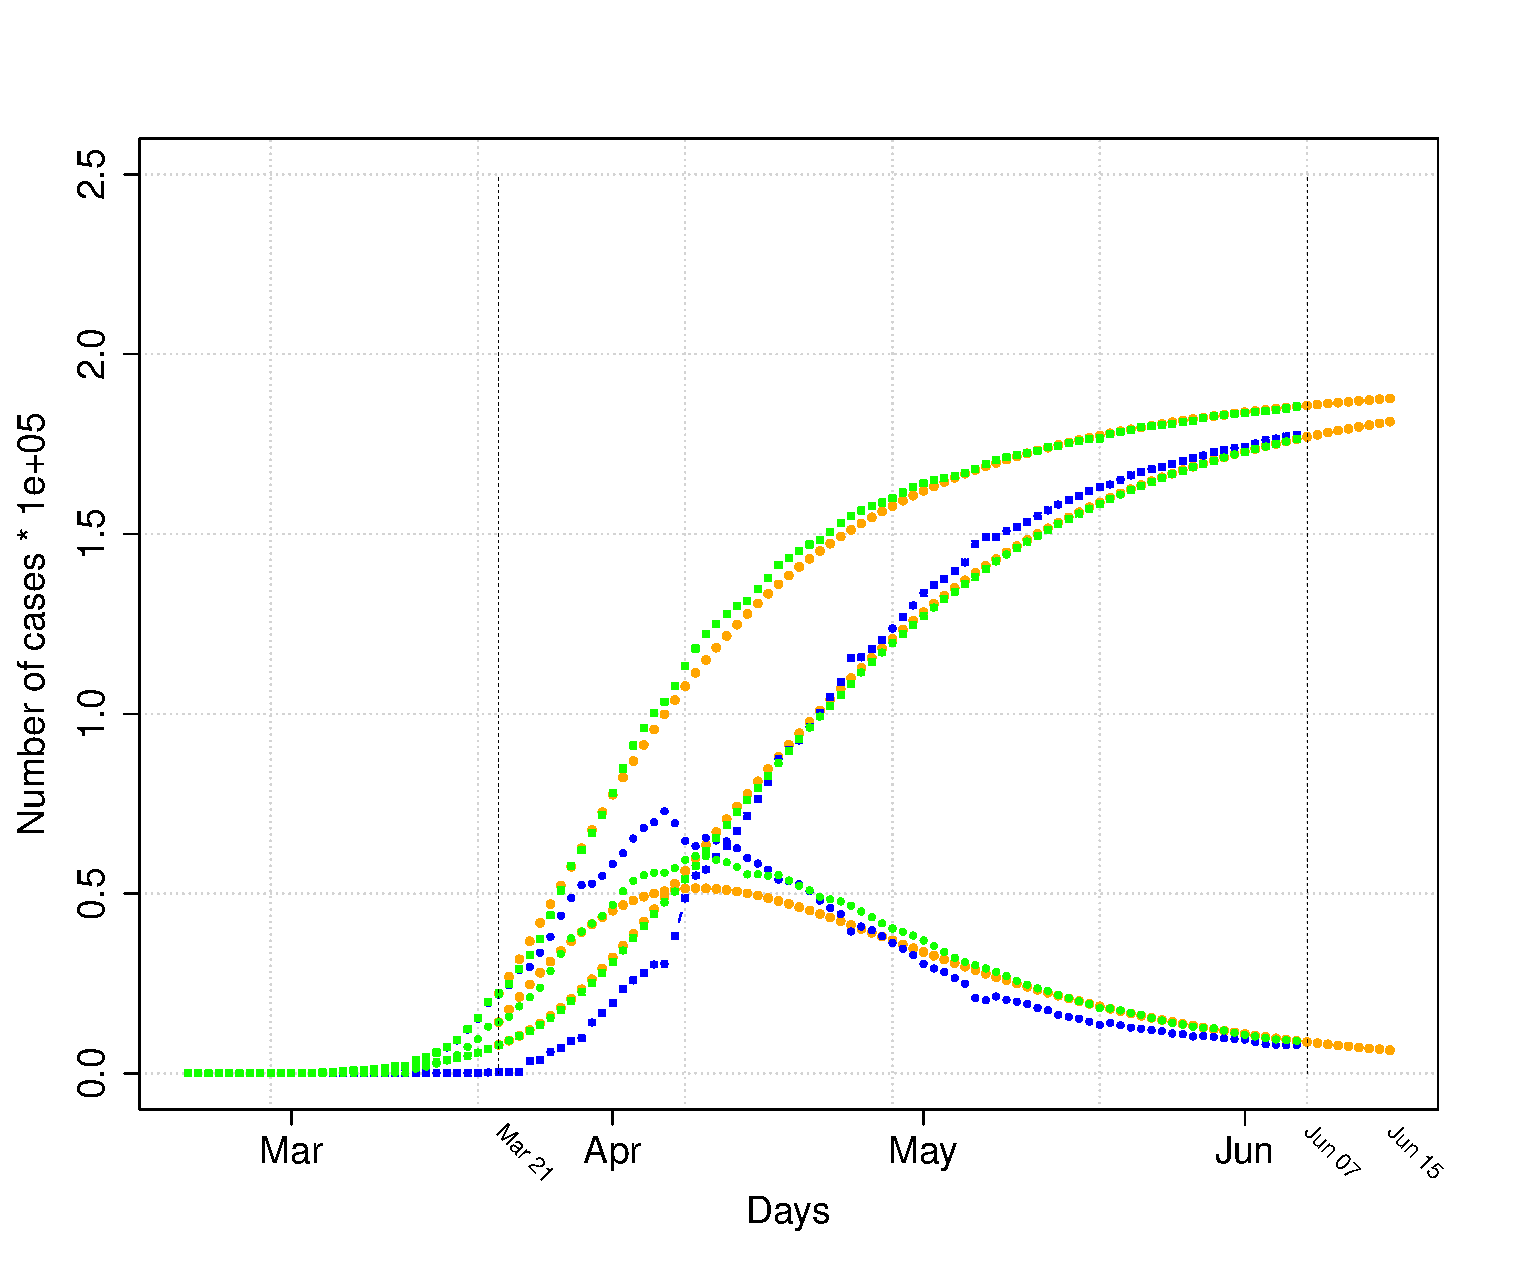
\includegraphics[width=2.5in,height=2in]{germany_figure_b_07_06_2020.eps}}
\end{center}
\begin{center}
\caption{SIR model, data pre-processing and RTT solution, Germany, March to June 2020
}
\label{fig:germany_sir_model_07_06_2020}
\end{center}
\end{figure}

\begin{figure}
\begin{center}
%\subfloat [Second-chance model and absolute standard normal]
{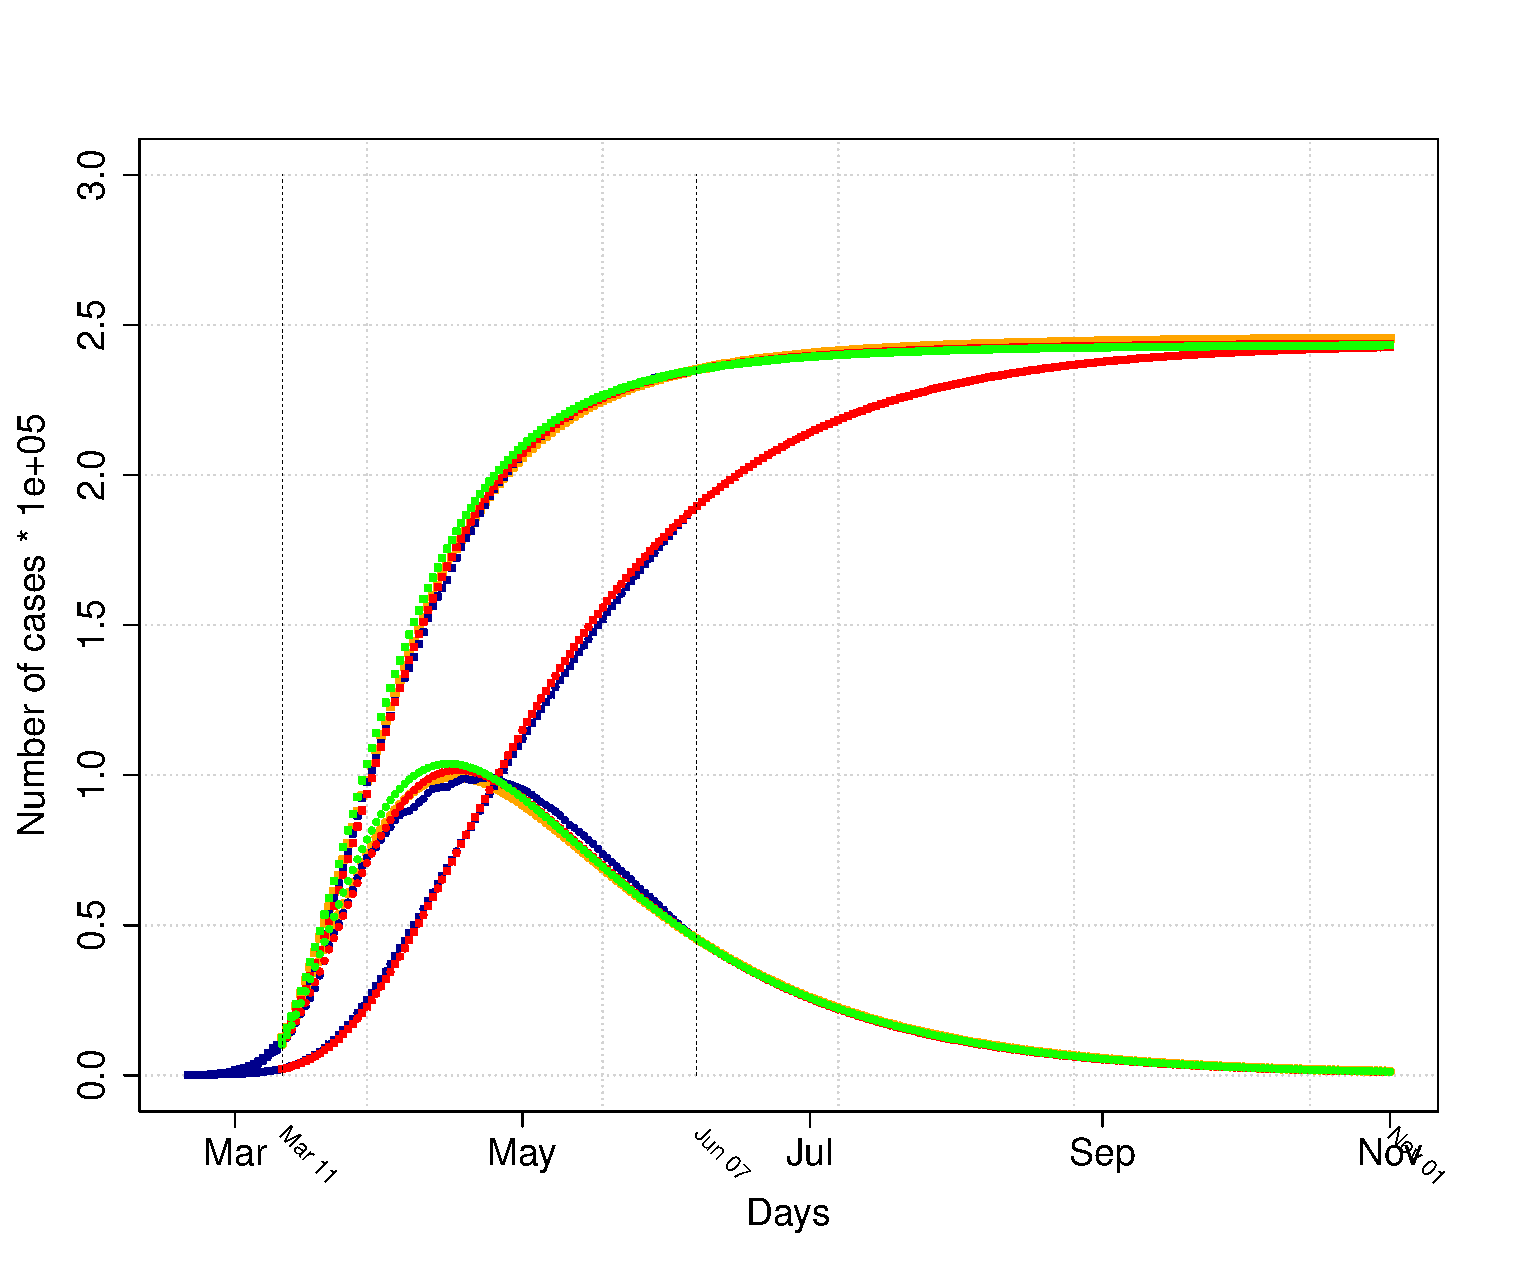
\includegraphics[width=2.5in,height=2in]{italy_figure_a_07_06_2020.eps}}
\qquad
{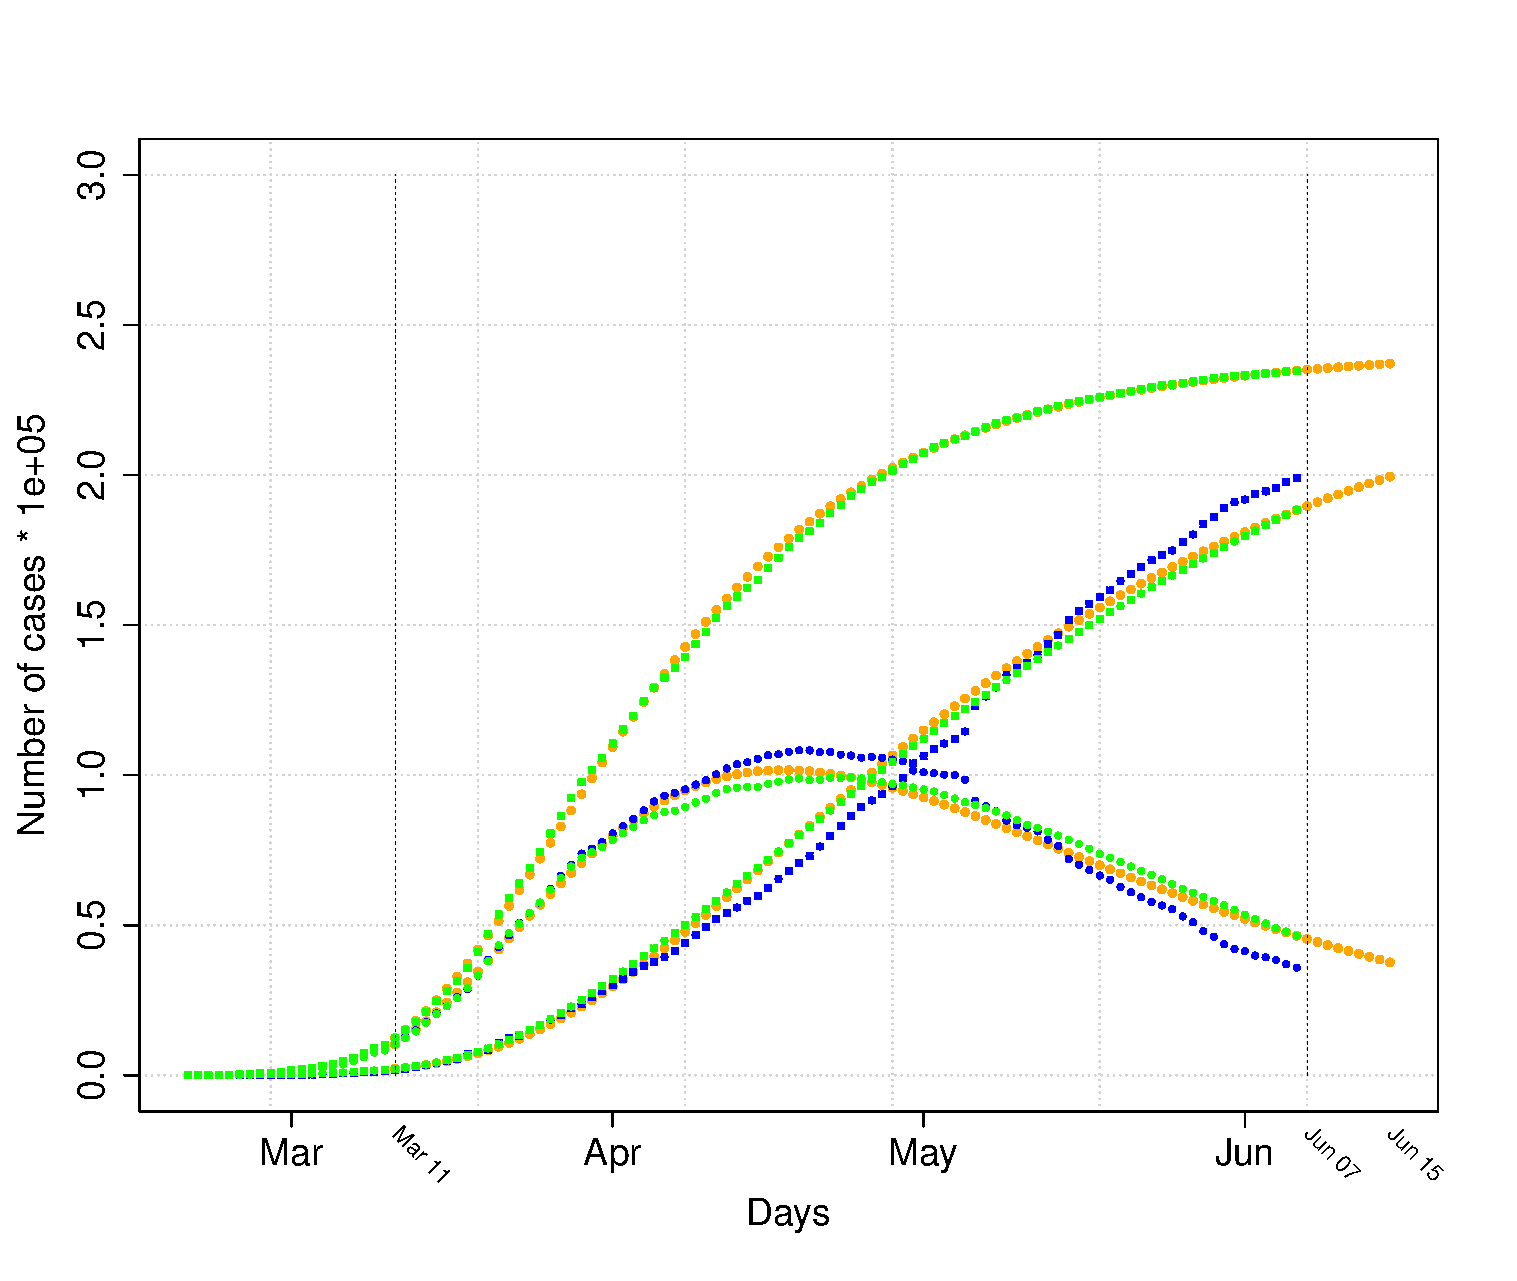
\includegraphics[width=2.5in,height=2in]{italy_figure_b_07_06_2020.eps}}
\end{center}
\begin{center}
\caption{SIR model, data pre-processing and RTT solution, Italy, March to June 2020
}
\label{fig:italy_sir_model_07_06_2020}
\end{center}
\end{figure}

\begin{figure}
\begin{center}
%\subfloat [Second-chance model and absolute standard normal]
{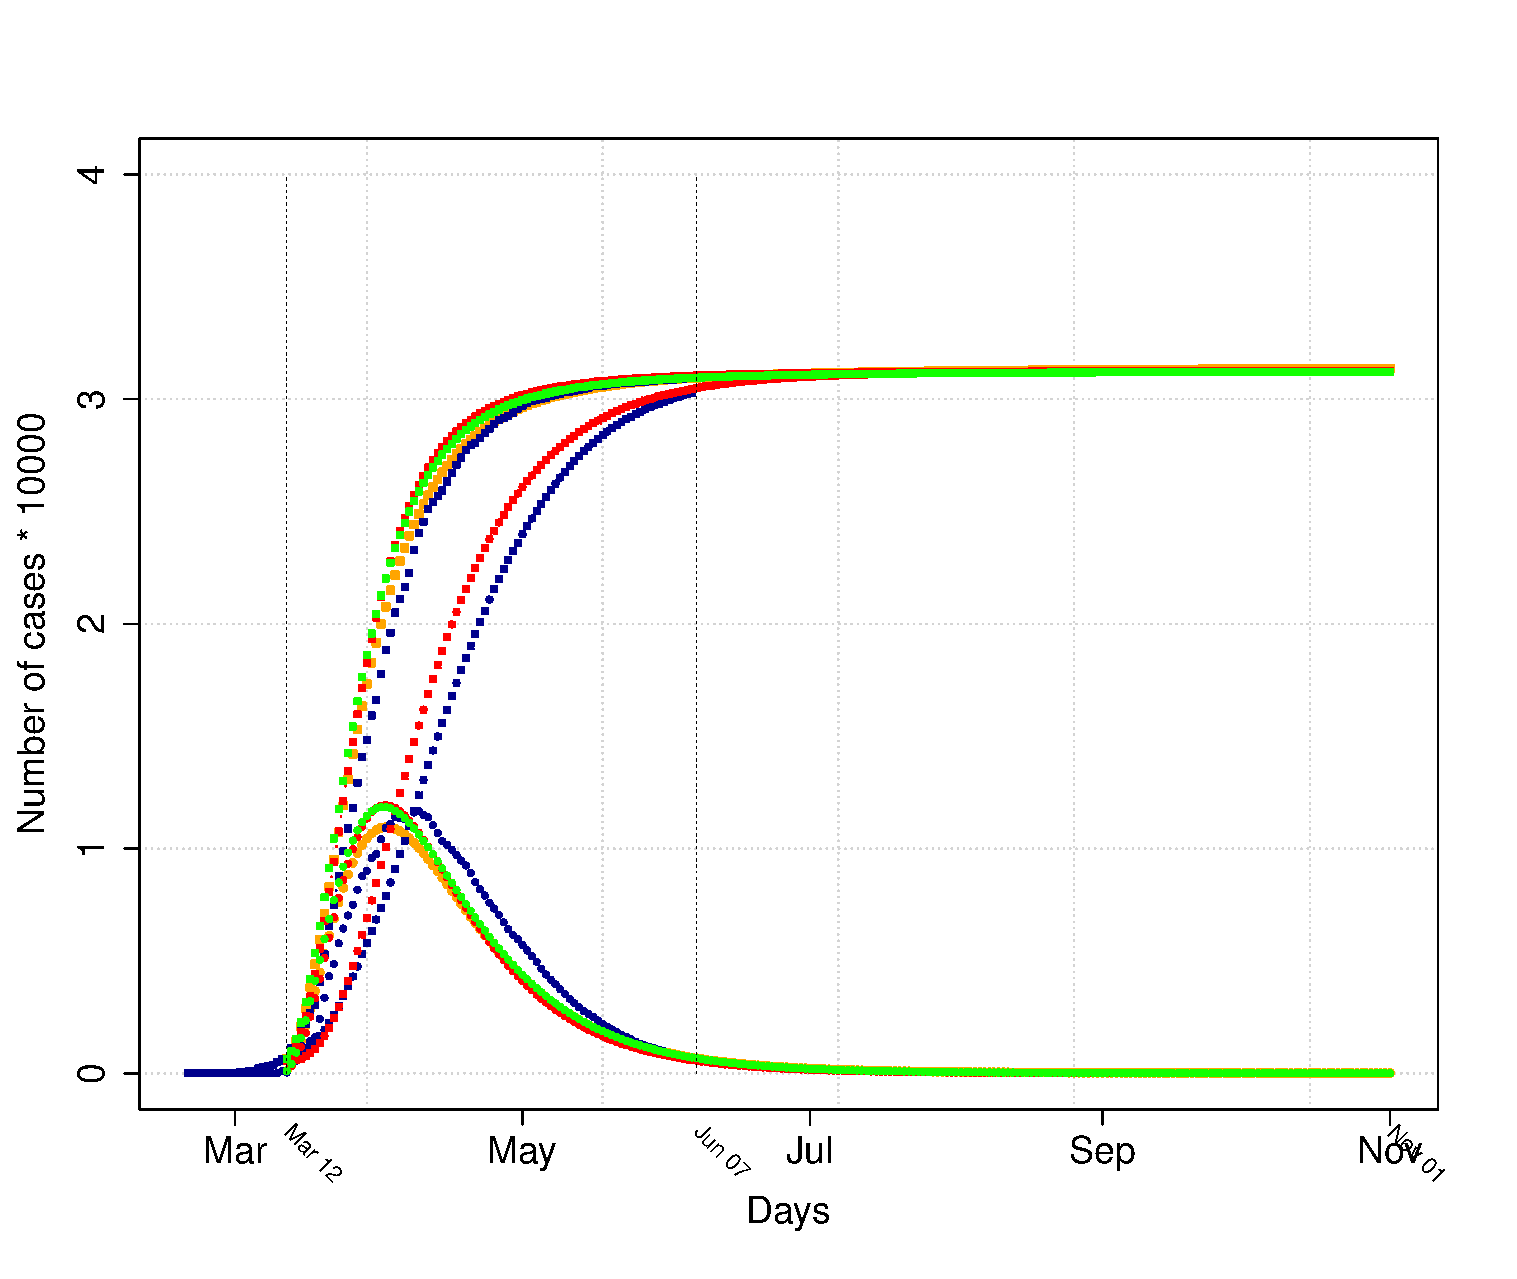
\includegraphics[width=2.5in,height=2in]{swiss_figure_a_07_06_2020.eps}}
\qquad
{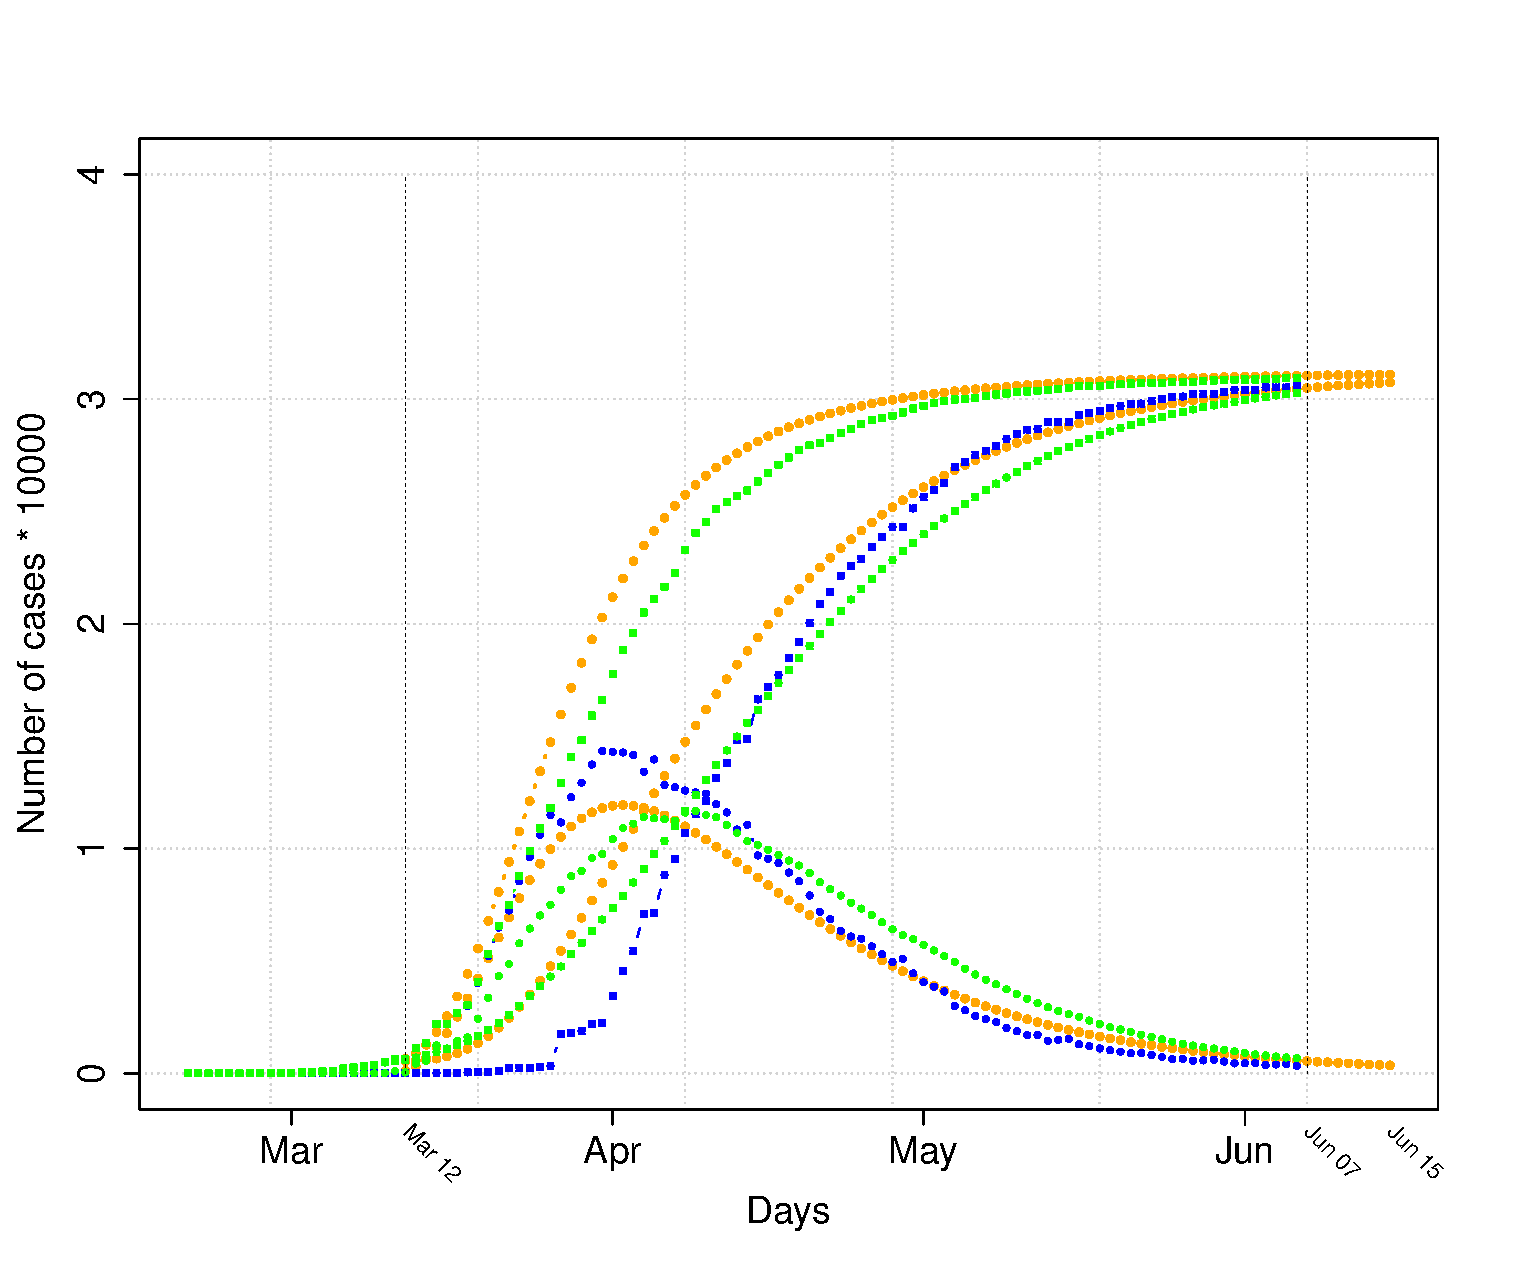
\includegraphics[width=2.5in,height=2in]{swiss_figure_b_07_06_2020.eps}}
\end{center}
\begin{center}
\caption{SIR model, data pre-processing and RTT solution, Switzerland, March to June 2020
}
\label{fig:swiss_sir_model_07_06_2020}
\end{center}
\end{figure}

\begin{figure}
\begin{center}
%\subfloat [Second-chance model and absolute standard normal]
{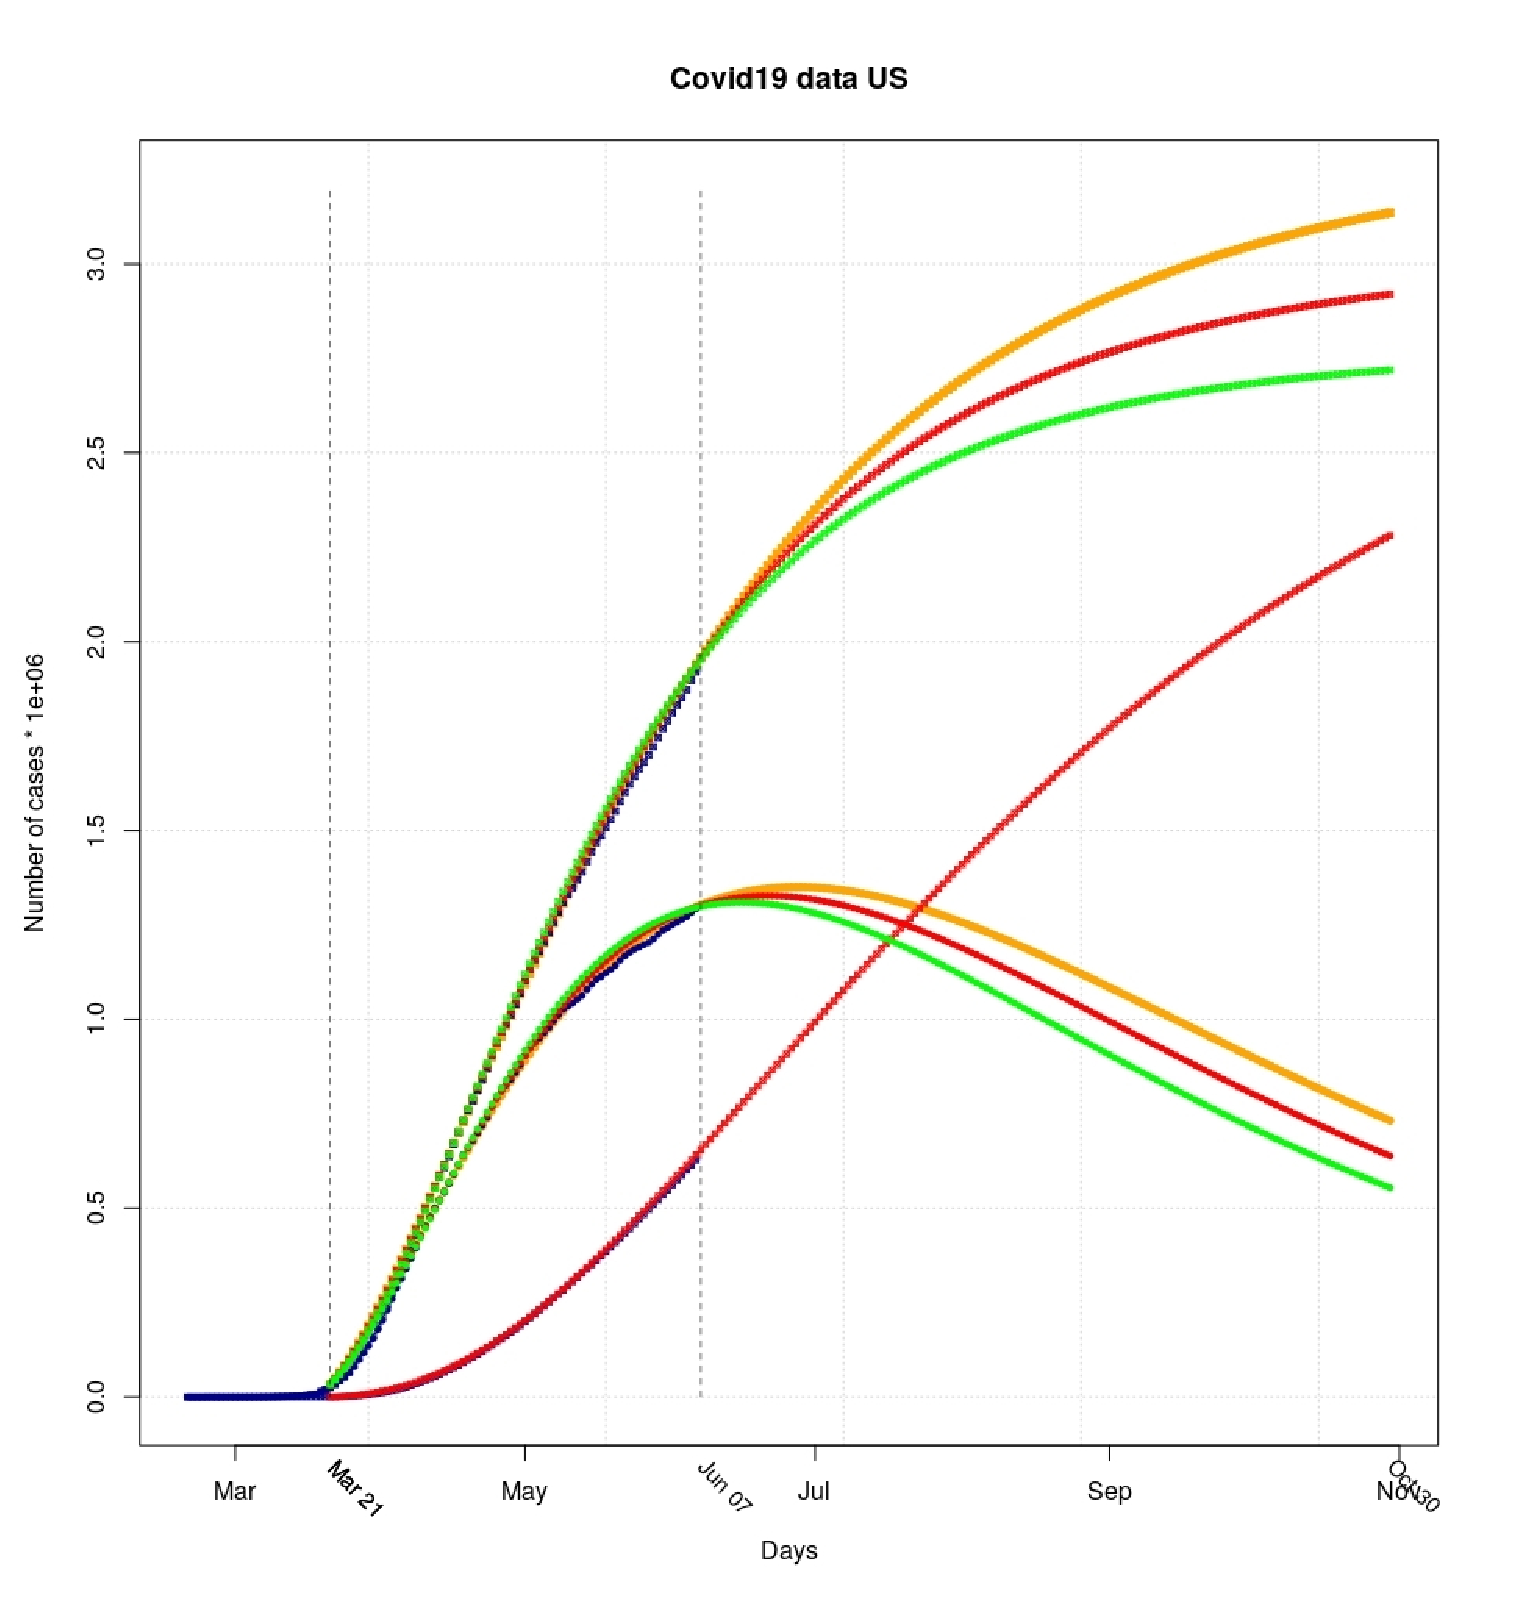
\includegraphics[width=2.5in,height=2in]{usa_figure_a_07_06_2020.eps}}
\qquad
{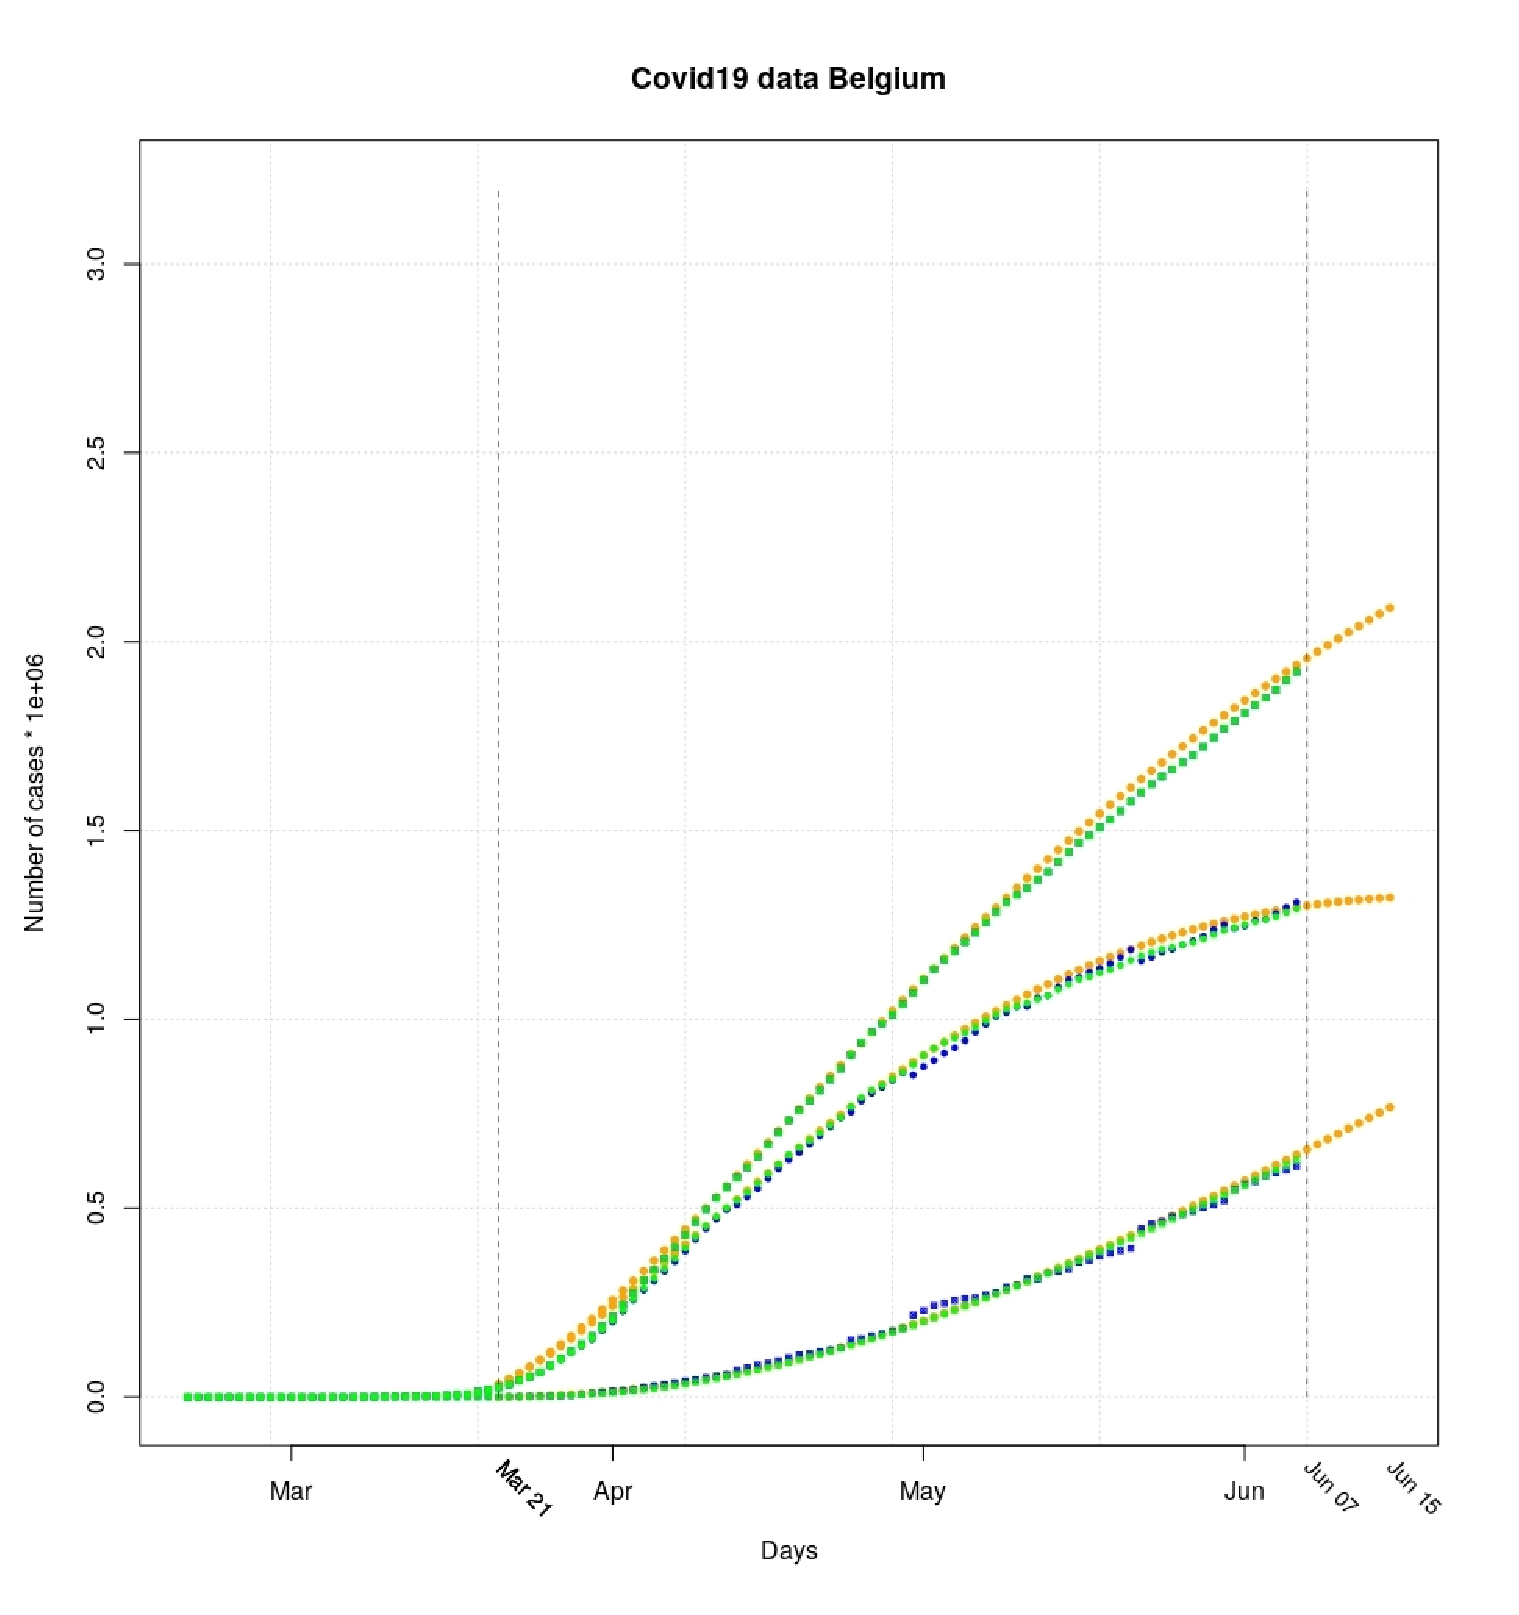
\includegraphics[width=2.5in,height=2in]{usa_figure_b_07_06_2020.eps}}
\end{center}
\begin{center}
\caption{SIR model, data pre-processing and RTT solution, USA, March to June 2020
}
\label{fig:usa_sir_model_07_06_2020}
\end{center}
\end{figure}



\section{A remark on incremental new cases} \label{More}

In principle, the increments $X(i)-X(i-1)$ should be independent, Poisson distributed with some local mean, provided by the differential equations. Poisson random variables $Z$, positive and with variance equal to the mean, should display when this mean is at least $5$ or so, the remarkable property that $\sqrt{Z}$ has standard deviation very close to, and fast converging to ${1 \over 2}$. Whether or not this theoretical fact is satisfied empirically by the $F(i)=\sqrt{max(1,X(i)-X(i-1))}$ data can be checked without reference to the differential equations. Simply, choose a window size $WS$ such as $5$ or $10$, do for each $i$ linear regression of $F(i-WS:i+WS)$ on time $(i-WS:i+WS)$, and record the averages and slopes or correlation coefficients of these lines as well as the standard deviations $\hat{\sigma_i}$ of the residuals. These standard deviations are supposed to estimate ${1 \over 2}$, or else assist in data diagnosis or identify a batch-size of arrivals. Italy and USA display weekly seasonality in which significantly less cases are reported on weekends, and delayed reporting could be more the rule than the exception. In any case, the empirical standard deviations $\hat{\sigma_i}$ are so much bigger than ${1 \over 2}$ that probabilistic modelling methods based on the Poisson hypothesis are not justified.


\section{Appendix 1: Correction of the number of infected cases}

Let $B$ be the $n$ by $n$ matrix with zeros above the diagonal and ones on and below the diagonal. Let $A$ be the $2 n$ by $n$ matrix that has $\gamma B$ in the first $n$ rows and $\gamma B$ plus the identity matrix in the last $n$ rows. Let $V$ be a column vector with $R$ in the top half and $X$ in the bottom half. The regression equation $A \hat{I} \approx V$
precisely expresses that $R$ should be $\beta$ times the cumulative sum of the $I$ values, and $X$ should be the latter vector (approximately $R$) plus $I$. The "regression coefficients" $\hat{I}$ are a compromise to manifest this requirement. Once determined, the removed cases are re-defined as $\hat{R}=X-\hat{I}$. The initial parts of the vectors $\hat{R}$ and $\hat{I}$ are further modified if necessary to prevent negative values or violation of monotonicity of $\hat{R}$.

\begin{figure}[H]
\begin{center}
%\subfloat [Second-chance model and absolute standard normal]
{\includegraphics[width=2.5in,height=2in]{chile.eps}}
\qquad
{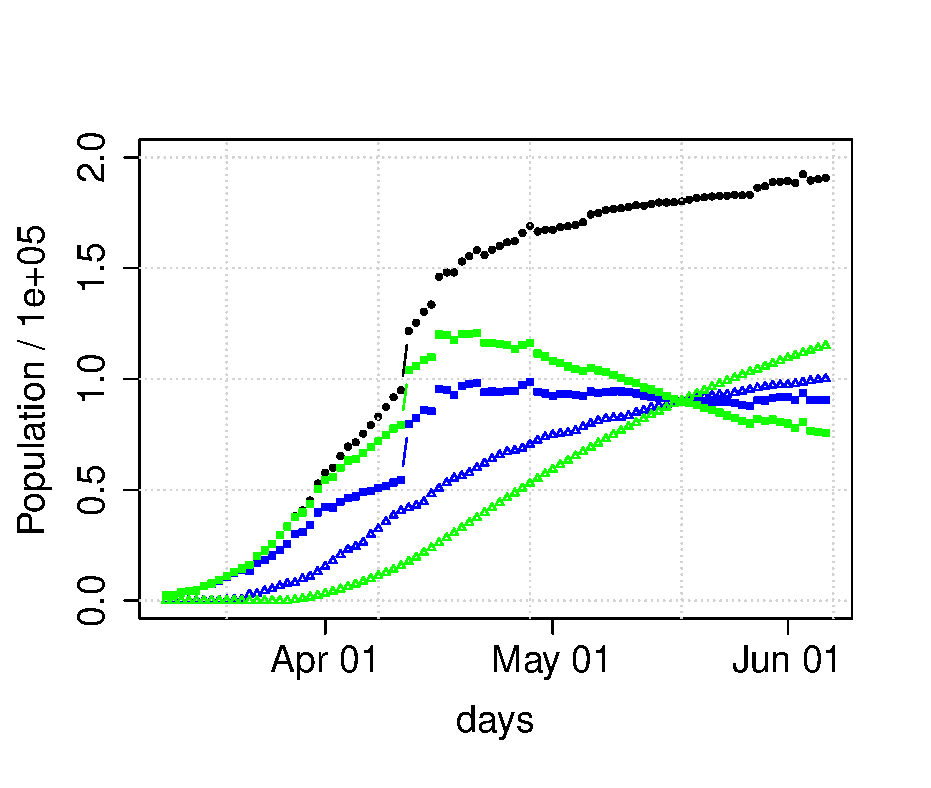
\includegraphics[width=2.5in,height=2in]{france.eps}}
\qquad
{\includegraphics[width=2.5in,height=2in]{india.eps}}
\qquad
{\includegraphics[width=2.5in,height=2in]{iran.eps}}
\end{center}
\begin{center}
\caption{Data pre-processing: Raw in blue, modified in green. Chile (top left), France (top right), India (bottom left) and Iran (bottom right), March to June 2020
}
\label{fig:chile_france_india_iran_07_06_2020}
\end{center}
\end{figure}

\begin{figure}[H]
    \begin{center}
%\subfloat [Second-chance model and absolute standard normal]
        {\includegraphics[width=2.5in,height=2in]{israel.eps}}
        \qquad
        {\includegraphics[width=2.5in,height=2in]{peru.eps}}
        \qquad
    {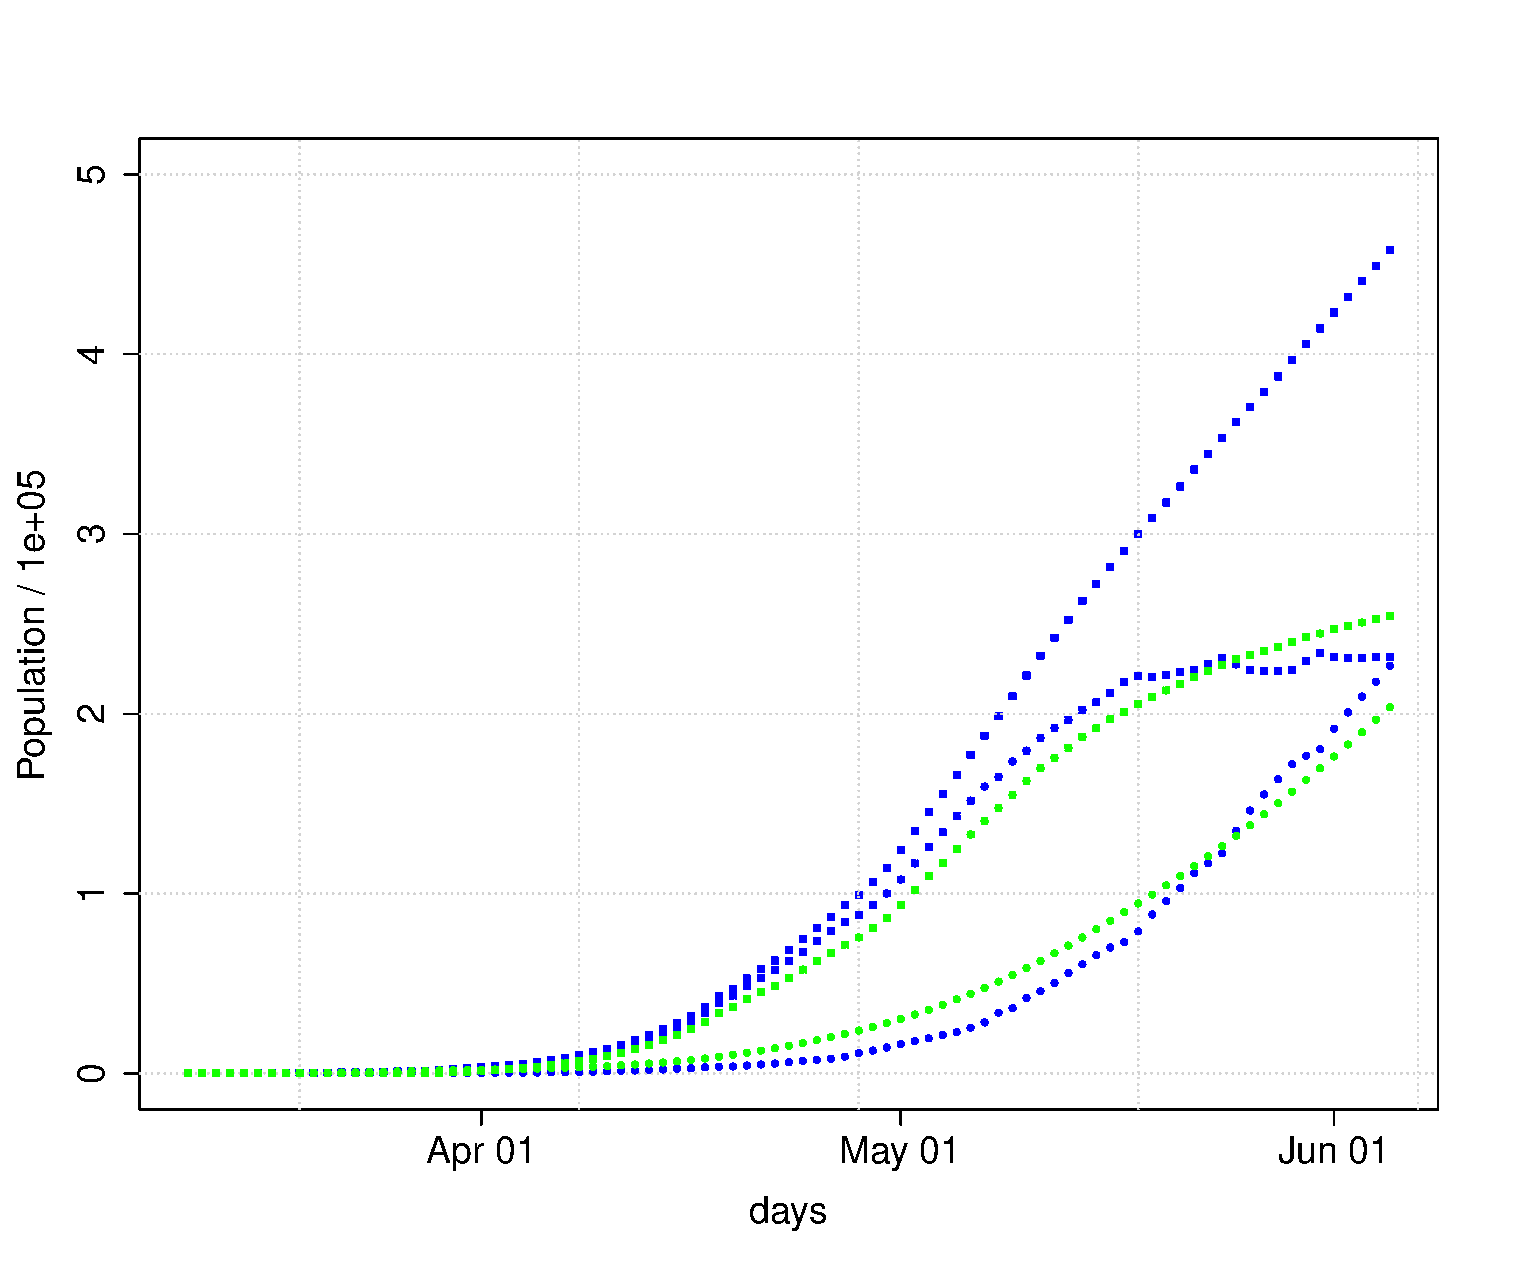
\includegraphics[width=2.5in,height=2in]{russia.eps}}
    \qquad
    {\includegraphics[width=2.5in,height=2in]{turkey.eps}}
    \end{center}
    \begin{center}
    \caption{Data pre-processing: Raw in blue, modified in green. Israel (top left), Peru (top right), Russia (bottom left) and Turkey (bottom right), March to June 2020
    }
\label{fig:israel_peru_russia_turkey_07_06_2020}
    \end{center}
\end{figure}


\begin{figure}[H]
    \begin{center}
%\subfloat [Second-chance model and absolute standard normal]
        {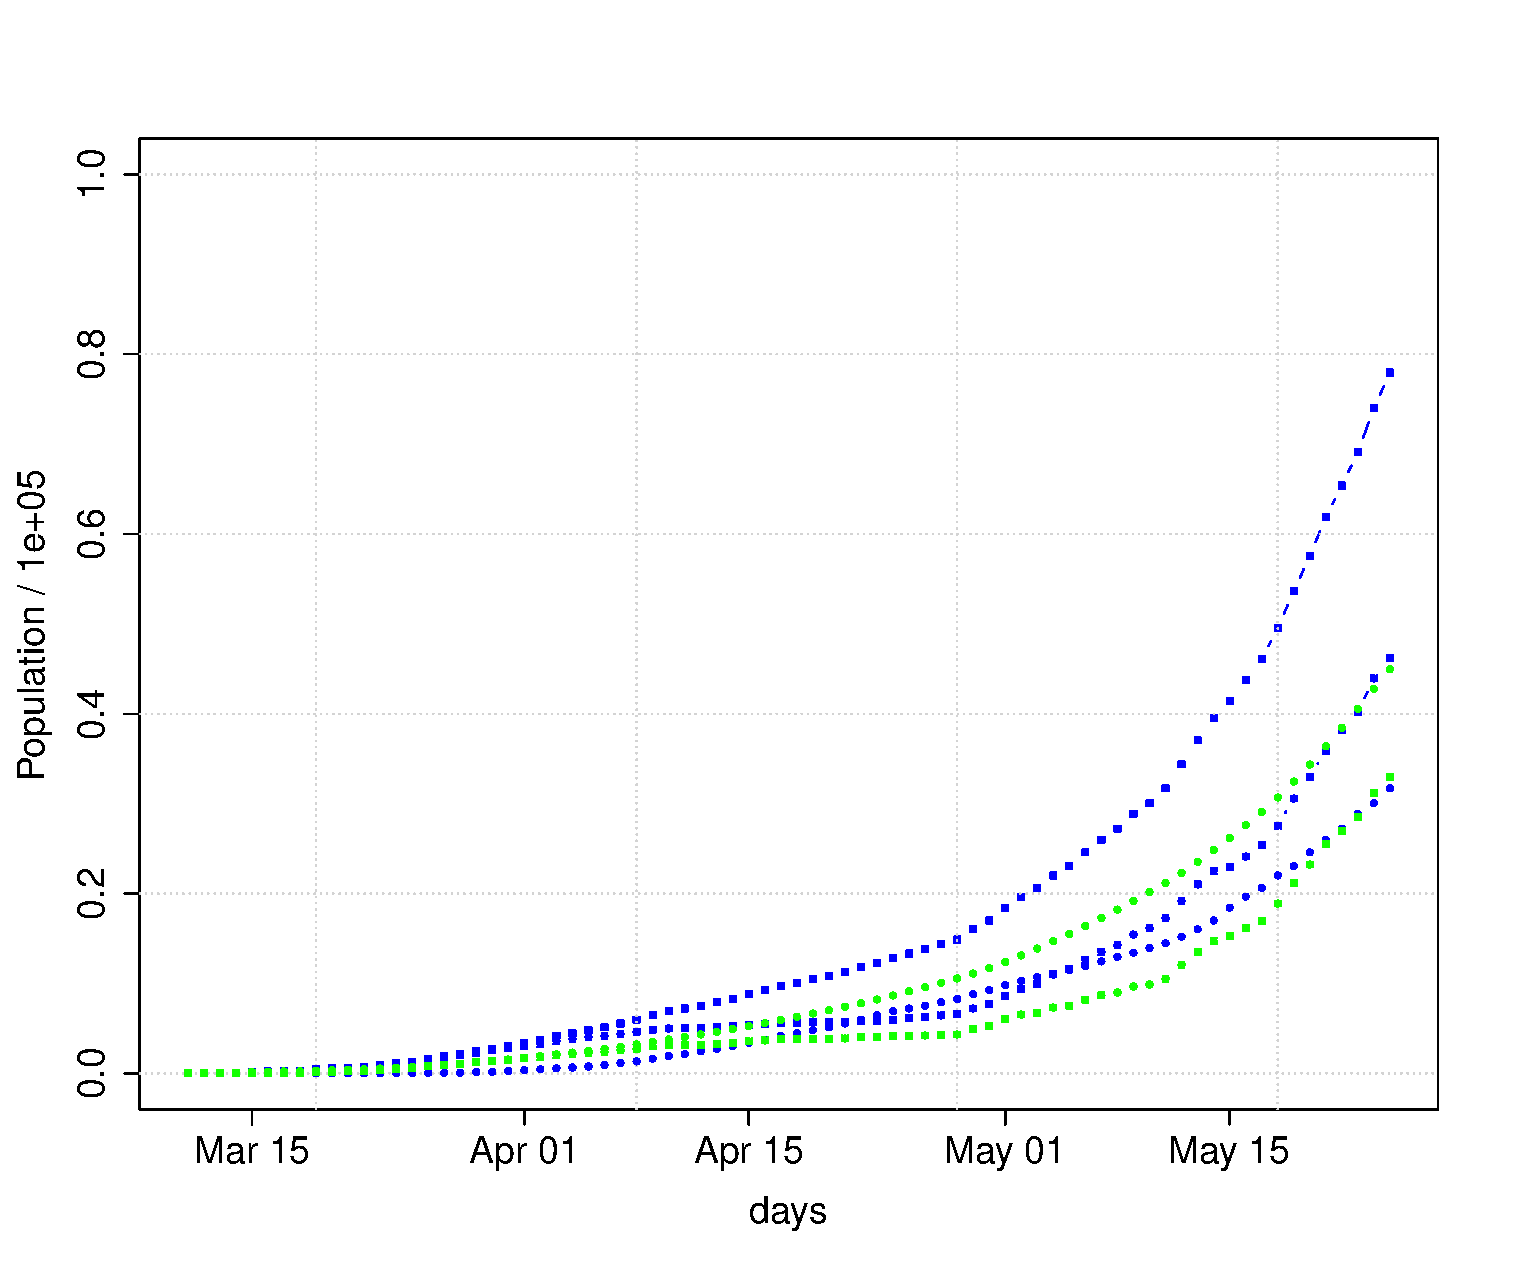
\includegraphics[width=2.5in,height=2in]{chile_25_05_2020.eps}}
        \qquad
        {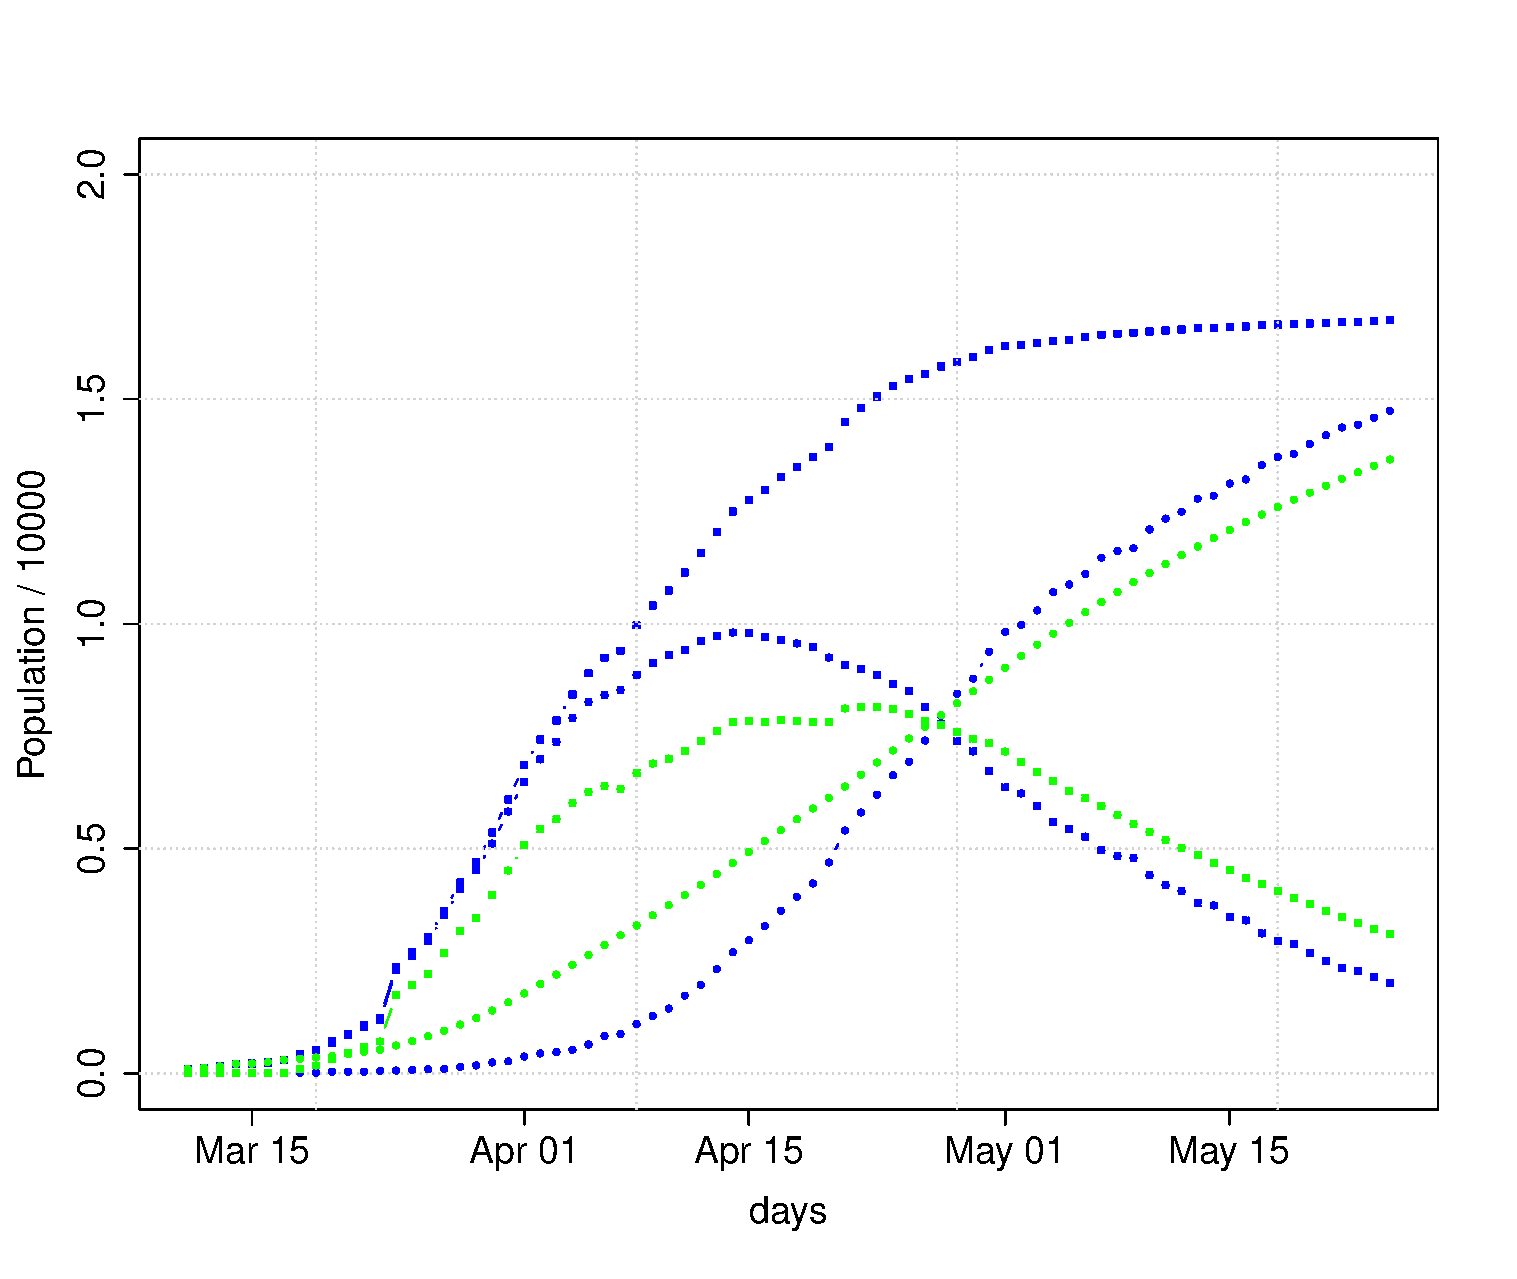
\includegraphics[width=2.5in,height=2in]{israel_25_05_2020.eps}}
    \end{center}
    \begin{center}
    \caption{Data pre-processing: Raw in blue, modified in green. Chile (left) and Israel (right), March to May 25th 2020
    }
\label{fig:chile_and_israel_25_05_2020}
    \end{center}
\end{figure}

\section{Appendix 2: A connection between RTT ande Diffusions}

If the processes $X$ and $R$ are diffusions and time increments are small enough, these processes behave locally as Brownian motions with drift given by the integrands in (\ref{thesolution}) and some diffusion coefficients. As such, the incremental random times (now denoted by $\tau$) are first passage times of Brownian motion, first hitting time of a constant height $D$, and as such have well known density functions, that could be used to build the likelihood model. In the benefit of simplicity and the ease with which the normal approximation handles dependent random times, we opted above for this inaccuracy, but first-passage densities are applied to.

This outlook allows for a deeper analysis. Let any of the two Brownian motions $B_t$ dealt with have local drift $\mu>0$ and standard deviation $\sigma$. Since $B_t - \mu t$ and $(B_t - \mu t)^2 - \sigma^2 t$ are mean-zero Martingales, their expected values at $\tau$ are zero too. This implies that $\tau$ has mean ${D \over \mu}$ and variance ${{\sigma^2 D} \over {\mu^3}}$. Hence, as in the application above $\tau$ has mean $1$ and constant variance, $\sigma$ must be proportional to $\mu$. So the stochastic differential equation corresponding to the deterministic differential equation (\ref{DEforX})-(\ref{DEforR}) has diffusion additions proportional to the drifts. Sticking to the assumption that sampling is frequent enough, the Fokker-Planck equations will lead to a likelihood function close to the Gaussian likelihood with exponential term (for the $X$-process, similarly for $R$)
\begin{equation}
    \exp\{-{1 \over {2 \sigma^2}}\sum ({{X(i+1)-X(i)} \over {{x({{i+1} \over \delta})-x({{i} \over \delta})}}}-1)^2\}
\end{equation}
and the corresponding denominator. The terms ${{x({{i+1} \over \delta})-x({{i} \over \delta})}}$ can be replaced by the mid-interval differentials (drifts) in (\ref{thesolution}).

The "corresponding denominator" in the SDE formulation, the product of the standard deviations appearing in the Gaussian density, is in fact identical to the Jacobian term of the RTT formulation, that views the data $(X,R)$ as coming as a transformation of variables of the Gaussian or first-passage times.

\bigskip

This Appendix concludes with some details on the first passage distribution. If $B_t$ is Brownian motion with drift $\mu>0$ and standard deviation $\sigma$, for every fixed $s \in {\cal R}$, 
\linebreak 
the process $\exp\{s (B_t - \mu t) - s^2 {{\sigma^2} \over 2} t\}$ is a mean-$1$ Martingale. Hence, the first hitting time $\tau$ of $D>0$ satisfies
\begin{equation} \label{firstpas1}
1 = E[\exp\{s (B_{\tau} - \mu \tau) - s^2 {{\sigma^2} \over 2} \tau  \}=\exp\{s D\} E[\exp\{-(\mu s +{{s^2 \sigma^2} \over 2})\tau\}]
\end{equation}
which becomes, upon the substitution $u=\mu s+{{s^2 \sigma^2} \over 2}$, (\textit{i.e.,} s = $\frac{\sqrt{({\mu \over \sigma})^2 +2 u}-{\mu \over \sigma}}{\sigma}$) the Laplace transform of the distribution of $\tau$
\begin{equation} \label{firstpas2}
E[\exp\{-u \tau\}]=\exp\{-{D \over \sigma}(\sqrt{({\mu \over \sigma})^2 +2 u}-{\mu \over \sigma})\}
\end{equation}

In principle, this formula, that can be found in Ricciardi \cite{Ricciardi} page 68, determines the distribution, but a formula for the density would be much in need. The cumulative distribution function of $\tau$ admits a very elegant formula in terms of the survival function $\Phi^*$ of the standard normal distribution, that can be found in Sacerdote and Giraudo \cite{Sacerdote}, formula (5.12).
\begin{equation} \label{firstpas3}
P(\tau \le t) = \Phi^*({D \over {\sigma \sqrt{t}}} - {\mu \over \sigma} \sqrt{t}) + \exp\{{{2 \mu D} \over \sigma^2}\} \Phi^*({D \over {\sigma \sqrt{t}}} + {\mu \over \sigma} \sqrt{t})
\end{equation}



\section*{Acknowledgements}

Thanks are due to Ilan Eshel from prompting this study and to Vahid
Bokharaie, Amit Huppert, Eytan Ruppin, Laura Sacerdote and David Steinberg for helpful suggestions.

The data analyzed in this work is taken from the COVID-19 Data Repository by
the Center for Systems Science and Engineering (CSSE) at Johns Hopkins
University.



\baselineskip= 28pt

\begin{thebibliography}{99}

\bibitem{Alon} Alon, N. (2019), The effect of drift change on Skorohod embedded distribution with applications in Finance. Master’s Thesis. Tel Aviv
University

\bibitem{Bassanetal} Bassan, B., Marcus, R., Meilijson, I. and Talpaz, H. (1997). Parameter erstimation in differential equations, using random time transformations. {\em Journal of the Italian Statistical Society}, {\bf 6}, 177--199.

\bibitem{Doeblin} Bru, B. and Yor, M. (2000). Comments on the life and mathematical legacy of Wolfgang Doeblin, {\em Finance and Stochastics}, {\bf 6}, 3–47.

\bibitem{Doeblin} Doeblin, W. (2000). "Sur l'équation de Kolmogoroff". {\em Comptes Rendus de l'Academie des Sciences}. 331. 

\bibitem{DubSch}  Dubins, L. E. and Schwarz, G. (1965). On continuous martingales. {\em Proceedings of the National Academy of Sciences}, {\bf 53}, 913–916.

\bibitem{Cuadras} Fortiana, J. and Cuadras, C. M. (1997). A family of matrices, the discretized brownian bridge, and distance-based regression. {\em Linear
Algebra and its Applications}, {\bf 264}, 173–-188.

\bibitem{AAA} Grenfell, B.T., Bj{\o}rnstad, O.N. and Filkenst\"{a}dt, B. A. (2002) Dynamics of Measles epidemics: scaling, noise, determinism and predictability with the TSIR model. {\em Ecological Monographs}, {\bf 72(2)}, 185-–202.

\bibitem{Karatzas} Karatzas, I. and Shreve, S. E. (1998). Brownian Motion and Stochastic Calculus. {\em Graduate texts in Mathematics}, Springer.

\bibitem{Kermack}  Kermack, W. O., McKendrick, A. G. (1927). A Contribution to the Mathematical Theory of Epidemics. {\em Proceedings of the Royal Society A}, {\bf 115 (772)}, 700-–721.

\bibitem{Krengel} Krengel, U. (1985). {\em Ergodic theorems}. de Gruyter.

\bibitem{Monroe} Monroe, I. (1987). Processes that can be embedded in Brownian Motion.
{\em The Annals of Probability}, {\bf 6 (1)}, 42--56

\bibitem{Murphy} Murphy, S. A. and  Van Der Vaart, A. W. (2000). On Profile Likelihood. {\em Journal of the American Statistical Association}. {\bf 95 (450)}, 127--138.

\bibitem{Ricciardi} Ricciardi, L. M. (1977). Diffusion processes and related topics in Biology. {\em Lecture Notes in Biomathematics}, Springer.

\bibitem{Sacerdote} Sacerdote, L. and Giraudo, M. T. (2013). Stochastic Integrate and Fire models: A review on mathematical methods and their applications. In Bachar M., Batzel J., Ditlevsen S. (eds), Stochastic Biomathematical Models. Lecture Notes in Mathematics, {\bf 2058}. Springer: Berlin, Heidelberg. 

\bibitem{Skorokhod} Skorokhod, A. V. (1965). Studies in the theory of random  processes. {\em Addison-Wesley}. 

\end{thebibliography}

\end{document}



